%! Author = Axel
%! Date = 26/09/2024

\documentclass[11pt]{article}

% Packages
\usepackage{amsmath}
\usepackage{amsfonts}
\usepackage{amssymb}
\usepackage{graphicx}
\usepackage{hyperref}
\usepackage{geometry}
\usepackage{forest}
\geometry{a4paper, margin=1in}
\usepackage{listing}
\usepackage{listings}

% Title, Author, and Date
\title{Metodologie di Programmazione}
\author{[Axel Rubini]}
\date{\today}

% Document
\begin{document}

\maketitle
\tableofcontents
\newpage

\section{Introduzione}
Appunti del corso di Metodologie di Programmazione, tenuto dal Prof. Stefano Faralli presso l'Università degli Studi di Roma "La Sapienza".

\section{Dati In Java}
\subsection{Tipi di dato}
Un tipo di dato è un insieme di valori e delle operazioni che possono essere eseguite su questi valori.
esempi:
\begin{itemize}
    \item \textbf{Intero}: rappresenta un numero intero.
    \item \textbf{Reale}: rappresenta un numero decimale.
    \item \textbf{Carattere}: rappresenta un singolo carattere.
    \item \textbf{Stringa}: rappresenta una sequenza di caratteri non é realmente un tipo di dato primitivo.
    \item \textbf{Booleano}: rappresenta un valore di verità, può essere vero o falso.
    \end{itemize}
i tidi di dati primitivi sono detti built-in, mentre i tipi di dati definiti dall'utente sono detti derived.
In java tutte le variabili devono essere dichiarate con un tipo di dato, essendo un linguaggio fortemente tipizzato.
non si puó dichiarare senze prima dichiararla.
Il nome assegnato ad una variabile é detto identificatore, in java gli identificatori sono case-sensitive.
si utilizzano le convenzioni di scrittura camelCase o snake\_case per gli identificatori.



\subsection{Conversioni di tipo}
Come convertire un tipo di dato in un altro?
da Stringa ad intero:
\begin{lstlisting}[language=Java]
public class SommaInteri {
    public static void main(String[] args) {
        String num1 = "10";
        String num2 = "20";
        int n1 = Integer.parseInt(num1);
        int n2 = Integer.parseInt(num2);
        System.out.println(n1 + n2);
    }
}
\end{lstlisting}
da stringa a reale:
\begin{lstlisting}[language=Java]
public class SommaReali {
    public static void main(String[] args) {
        String num1 = "10.5";
        String num2 = "20.5";
        double n1 = Double.parseDouble(num1);
        double n2 = Double.parseDouble(num2);
        System.out.println(n1 + n2);
    }
}
\end{lstlisting}

Java definisce l'ooperatore + sul tipo di dato "built-in" Stringa, questo operatore viene utilizzato per concatenare le stringhe.
Quando si utilizza l'operatore + con una stringa e un altro tipo di dato, il risultato sarà una stringa.
\begin{lstlisting}[language=Java]
public class ConcatenazioneStringhe {
    public static void main(String[] args) {
        String nome = "Mario";
        int eta = 30;
        System.out.println("Ciao mi chiamo " + nome + " e ho " + eta + " anni");
    }
}
\end{lstlisting}

\subsubsection{caratteri e stringhe}
In java il tipo di dato char rappresenta un singolo carattere, mentre il tipo di dato String rappresenta una sequenza di caratteri.
\begin{lstlisting}[language=Java]
public class CaratteriStringhe {
    public static void main(String[] args) {
        char carattere = 'a';
        String stringa = "ciao";
        System.out.println(carattere);
        System.out.println(stringa);
    }
}
\end{lstlisting}
ci sono poi caratteri di escape come:
\begin{itemize}
    \item \textbf{\textbackslash n}: new line
    \item \textbf{\textbackslash t}: tab
    \item \textbf{\textbackslash "}: doppio apice
    \item \textbf{\textbackslash \textbackslash}: backslash
    \end{itemize}
\subsubsection{booleano}
Il tipo di dato booleano rappresenta un valore di verità, può essere vero o falso.
\begin{lstlisting}[language=Java]
public class Booleano {
    public static void main(String[] args) {
        boolean b1 = true;
        boolean b2 = false;
        System.out.println(b1);
        System.out.println(b2);
    }
}
\end{lstlisting}
gli operatori logici sono:
\begin{itemize}
    \item \textbf{\&\&}: and
    \item \textbf{||}: or
    \item \textbf{!}: not
    \end{itemize}
\subsubsection{operatori di confronto}
Gli operatori di confronto permettono di confrontare due valori e restituiscono un valore booleano.
gli operatori di confronto sono:
\begin{itemize}
    \item \textbf{==}: uguale
    \item \textbf{!=}: diverso
    \item \textbf{>}: maggiore
    \item \textbf{<}: minore
    \item \textbf{>=}: maggiore o uguale
    \item \textbf{<=}: minore o uguale
    \end{itemize}
\subsubsection{Consapevolezza del tipo di dato}
In java é importante essere consapevoli del tipo di dato con cui si sta lavorando, poiché le operazioni che si possono eseguire su un tipo di dato dipendono dal tipo di dato stesso.
\begin{lstlisting}[language=Java]
public class ConsapevolezzaTipoDato {
    public static void main(String[] args) {
        int n1 = 10;
        int n2 = 20;
        System.out.println(n1 + n2); // somma
        System.out.println(n1 + " " + n2); // concatenazione
    }
}
\end{lstlisting}
Le conversioni di tipo possono essere utili per convertire un tipo di dato in un altro, ma bisogna fare attenzione a non perdere informazioni durante la conversione.
esistono diversi modi per convertire un tipo:
\begin{itemize}
    \item \textbf{Casting esplicito}: si utilizza il casting esplicito per convertire un tipo di dato in un altro, ma bisogna fare attenzione a non perdere informazioni durante la conversione.
    \begin{lstlisting}[language=Java]
public class CastingEsplicito {
    public static void main(String[] args) {
        double d = 10.5;
        int i = (int) d;
        System.out.println(i);
    }
}
\end{lstlisting}
si puó perdere precisione durante la conversione.
    \item \textbf{Conversione implicita}: Java esegue la conversione implicita quando si assegna un valore di un tipo di dato più piccolo a un tipo di dato più grande.
    \begin{lstlisting}[language=Java]
public class ConversioneImplicita {
    public static void main(String[] args) {
        int i = 10;
        double d = i;
        System.out.println(d);
    }
}
\end{lstlisting}
    essendo l'intero un tipo di dato più piccolo del reale, java esegue la conversione implicita.
    \item \textbf{Conversione esplicita}: Integer.parseInt() per convertire una stringa in un intero,Doube.parseDouble() per convertire una stringa in un reale.
    \end{itemize}

\section{JRE e JDK}
JRE (Java Runtime Environment) è l'ambiente di esecuzione di Java, che include la JVM (Java Virtual Machine) e le librerie di runtime necessarie per eseguire un'applicazione Java.
JDK (Java Development Kit) è il kit di sviluppo di Java, che include il JRE e gli strumenti di sviluppo necessari per creare, compilare e testare un'applicazione Java.
Per sviluppare un'applicazione Java, è necessario installare il JDK sul proprio computer.
\section{Hello World}
\begin{lstlisting}[language=Java]
public class HelloWorld {
    public static void main(String[] args) {
        System.out.println("Hello, World!");
    }
}
\end{lstlisting}
\section{Programmazione Orientata agli Oggetti}
La programmazione orientata agli oggetti (OOP) è un paradigma di programmazione che si basa sul concetto di "oggetto", che rappresenta un'istanza di una classe.
Le classi sono i "mattoni" fondamentali della programmazione orientata agli oggetti, e vengono utilizzate per definire gli oggetti e le loro proprietà.
Le proprietà di un oggetto sono definite da variabili di istanza, mentre i comportamenti di un oggetto sono definiti da metodi.
\section{Classi e Oggetti}
Una classe è un modello che definisce le proprietà e i comportamenti di un oggetto.
Un oggetto è un'istanza di una classe, che rappresenta un'entità del mondo reale.
La classe é il prototipo dell'oggetto, mentre l'oggetto é una entitá all'interno del programma, una ulteriore distinzione é che la classe é un tipo di dato definito dall'utente, mentre l'oggetto é un'istanza di un tipo di dato definito dall'utente.

\begin{lstlisting}[language=Java]
// Definizione della classe Persona
public class Persona {
    // Proprietà della classe Persona
    String nome;
    int eta;

    // Metodo per salutare
    public void saluta() {
        System.out.println("Ciao, mi chiamo " + nome);
    }
}

// Creazione di un oggetto della classe Persona
public class Main {
    public static void main(String[] args) {
        // Creazione di un oggetto persona1
        Persona persona1 = new Persona();
        // Inizializzazione delle proprietà dell'oggetto persona1
        persona1.nome = "Mario";
        persona1.eta = 30;

        // Utilizzo del metodo saluta dell'oggetto persona1
        persona1.saluta();
    }
}
\end{lstlisting}
per cui é il programma che crea l'oggetto, l'oggetto é un'istanza della classe, l'oggetto é un'entitá all'interno del programma.

\subsection{Campi}
I campi di una classe sono le variabili di istanza che rappresentano le proprietà dell'oggetto.
I campi di una classe possono essere di diversi tipi di dati, come interi, reali, caratteri, stringhe, booleani, ecc.
i campi di una classe sono in genere dichiarati come privati per garantire l'incapsulamento e l'accesso controllato alle proprietà dell'oggetto.
\begin{lstlisting}[language=Java]
public class Persona {
    // Campi della classe Persona
    private String nome;
    private int eta;

    // Metodi getter e setter per i campi della classe Persona
    public String getNome() {
        return nome;
    }

    public void setNome(String nome) {
        this.nome = nome;
    }

    public int getEta() {
        return eta;
    }

    public void setEta(int eta) {
        this.eta = eta;
    }
}
\end{lstlisting}
la sintassi per dichiarare un campo é:
private [static] [final] tipo nomeCampo [= valoreIniziale];
\begin{itemize}
    \item \textbf{private}: il campo è accessibile solo all'interno della classe.
    \item \textbf{static}: il campo è condiviso da tutte le istanze della classe.
    \item \textbf{final}: il campo è costante e non può essere modificato.
    \item \textbf{tipo}: il tipo di dato del campo.
    \item \textbf{nomeCampo}: il nome del campo.
    \item \textbf{valoreIniziale}: il valore iniziale del campo se non dichiarato quando viene creato l'oggetto vengono assegnati dei valori di default nei casi di tipo di dato primitivo altrimenti in caso di altri oggetti viene assegnato il valore null.
    \end{itemize}
\subsection{Metodi}
\begin{itemize}
    \item \textbf{Metodi di istanza}: i metodi che operano sulle proprietà dell'oggetto.
    \item \textbf{Metodi statici}: i metodi che non operano sulle proprietà dell'oggetto.
    \item \textbf{Costruttori}: i metodi speciali che vengono utilizzati per inizializzare un oggetto.
\end{itemize}
\begin{lstlisting}[language=Java]
public class Persona {
    // Campi della classe Persona
    private String nome;
    private int eta;

    // Costruttore della classe Persona
    public Persona(String nome, int eta) {
        this.nome = nome;
        this.eta = eta;
    }

    // Metodo per salutare
    public void saluta() {
        System.out.println("Ciao, mi chiamo " + nome);
    }
}
\end{lstlisting}
la sintassi per dichiarare un metodo é:
[modificatore] [static] [tipoRitorno] nomeMetodo([parametri]) { corpoMetodo }
\begin{itemize}
    \item \textbf{modificatore}: il modificatore di accesso del metodo (public, private, protected, package-private).
    \item \textbf{static}: il metodo è condiviso da tutte le istanze della classe.
    \item \textbf{tipoRitorno}: il tipo di dato restituito dal metodo void nel caso non restituisce un valore.
    \item \textbf{nomeMetodo}: il nome del metodo.
    \item \textbf{parametri}: i parametri del metodo.
    \item \textbf{corpoMetodo}: il corpo del metodo.
\end{itemize}
\subsubsection{Costruttori}
\begin{itemize}
    \item I costruttori sono metodi speciali che vengono utilizzati per inizializzare un oggetto.
    \item Il costruttore ha lo stesso nome della classe e non ha un tipo di ritorno.
    \item Il costruttore può avere parametri per inizializzare le proprietà dell'oggetto.
    \item Se non viene definito un costruttore per una classe, Java fornisce un costruttore di default senza parametri.
    \item Se viene definito un costruttore per una classe, il costruttore di default non viene fornito da Java.
    \item Un costruttore può chiamare un altro costruttore della stessa classe utilizzando la parola chiave this.
\end{itemize}
\begin{lstlisting}[language=Java]
public class Persona {
    // Campi della classe Persona
    private String nome;
    private int eta;

    // Costruttore di default della classe Persona
    public Persona() {
        this.nome = "Mario";
        this.eta = 30;
    }

    // Costruttore della classe Persona
    public Persona(String nome, int eta) {
        this.nome = nome;
        this.eta = eta;
    }
}
\end{lstlisting}
\subsubsection{Chiamata di un metodo}
\begin{lstlisting}[language=Java]
public class Main {
    public static void main(String[] args) {
        // Creazione di un oggetto persona1
        Persona persona1 = new Persona("Mario", 30);
        // Utilizzo del metodo saluta dell'oggetto persona1
        persona1.saluta();
    }
}
\end{lstlisting}
\subsection{Differenza tra variabili locali e campi}
\begin{itemize}
    \item \textbf{Variabili locali}: le variabili definite all'interno di un metodo sono chiamate variabili locali.
    \item \textbf{Campi}: le variabili definite all'interno di una classe sono chiamate campi.
    \item \textbf{Variabili locali}: le variabili locali devono essere inizializzate prima di essere utilizzate.
    \item \textbf{Campi}: i campi vengono inizializzati con valori di default se non vengono inizializzati esplicitamente.
    \item \textbf{Variabili locali}: le variabili locali hanno uno scope limitato al blocco in cui sono definite.
    \item \textbf{Campi}: i campi hanno uno scope limitato all'intera classe.
\end{itemize}

\section{Incapsulamento e inizializzazione di default}
\subsection{Incapsulamento}
\begin{itemize}
    \item \textbf{Incapsulamento}: l'incapsulamento è il concetto di nascondere i dettagli di implementazione di un oggetto e fornire un'interfaccia per interagire con esso.
    \item \textbf{Campi privati}: i campi di una classe dovrebbero essere dichiarati come privati per garantire l'incapsulamento.
    \item \textbf{Metodi getter e setter}: i metodi getter e setter vengono utilizzati per accedere e modificare i campi privati di una classe.
    \item \textbf{Vantaggi dell'incapsulamento}: l'incapsulamento aiuta a mantenere l'integrità dei dati, a nascondere i dettagli di implementazione e a semplificare la manutenzione del codice.
\end{itemize}
Una classe interagisce con un'altra classe attraverso i metodi pubblici e costruttori. per cui bisogna fare affidamento sulle interfacce pubbliche di una classe per interagire con essa.
\subsubsection{Inizializzazione Implicita}
\begin{itemize}
    \item \textbf{Inizializzazione implicita}: i campi di una classe vengono inizializzati con valori di default se non vengono inizializzati esplicitamente.
    \item \textbf{Valori di default}: \begin{itemize}
        \item \textbf{Intero}: 0
        \item \textbf{Reale}: 0.0
        \item \textbf{Carattere}: '\textbackslash u0000'
        \item \textbf{Stringa}: null
        \item \textbf{Booleano}: false
        \end{itemize}
    \item \textbf{Valori di default per riferimenti}: i valori di default per i riferimenti sono null.
    \item \textbf{Valori di default per array}: i valori di default per gli array sono null.
\end{itemize}
\section{La classe String}
\subsection{Stringhe in Java}
String é una classe fondamentale in Java, che rappresenta una sequenza di caratteri.
Le stringhe in Java sono immutabili, il che significa che non possono essere modificate una volta create.
Java fornisce una serie di metodi per manipolare le stringhe, come la concatenazione, la ricerca, la sostituzione, ecc.
\subsection{Operazioni sulle Stringhe}
\begin{itemize}
    \item \textbf{Concatenazione}: la concatenazione di stringhe viene eseguita utilizzando l'operatore + o il metodo concat().
    \item \textbf{Lunghezza}: il metodo length() restituisce la lunghezza di una stringa.
    \item \textbf{Confronto}: i metodi equals() e equalsIgnoreCase() vengono utilizzati per confrontare le stringhe.
    \item \textbf{Ricerca}: i metodi indexOf() e lastIndexOf() vengono utilizzati per cercare una sottostringa all'interno di una stringa.
    \item \textbf{Sostituzione}: il metodo replace() viene utilizzato per sostituire una sottostringa con un'altra.
    \item \textbf{Maiuscole e minuscole}: i metodi toUpperCase() e toLowerCase() vengono utilizzati per convertire una stringa in maiuscolo o minuscolo.
    \item \textbf{Trim}: il metodo trim() viene utilizzato per rimuovere gli spazi bianchi in eccesso da una stringa.
    \item \textbf{Substring}: il metodo substring() viene utilizzato per estrarre una sottostringa da una stringa.
    \item \textbf{Split}: il metodo split() viene utilizzato per suddividere una stringa in base a un delimitatore.
    \item \textbf{Format}: il metodo format() viene utilizzato per formattare una stringa.
\end{itemize}
\subsection{StringBuilder e StringBuffer}
Se si deve manipolare una stringa in modo intensivo, è consigliabile utilizzare la classe StringBuilder o StringBuffer.
\begin{itemize}
    \item \textbf{StringBuilder}: la classe StringBuilder non é sincronizzata e più efficiente in termini di prestazioni.
    \item \textbf{StringBuffer}: la classe StringBuffer è sincronizzata e più sicura in un ambiente multithreading.
\end{itemize}
esempio di utilizzo di StringBuilder:
\begin{lstlisting}[language=Java]
public class StringBuilderExample {
    public static void main(String[] args) {
        StringBuilder sb = new StringBuilder();
        sb.append("Hello");
        sb.append(" ");
        sb.append("World");
        System.out.println(sb.toString());
    }
}
\end{lstlisting}
\subsection{Confrontare Stringhe}
\begin{itemize}
    \item \textbf{equals()}: il metodo equals() viene utilizzato per confrontare due stringhe in base al contenuto.
    \item \textbf{==}: l'operatore == viene utilizzato per confrontare due stringhe in base all'indirizzo di memoria.
    \item \textbf{equalsIgnoreCase()}: il metodo equalsIgnoreCase() viene utilizzato per confrontare due stringhe ignorando le differenze tra maiuscole e minuscole.
    \item \textbf{compareTo()}: il metodo compareTo() viene utilizzato per confrontare due stringhe in base all'ordine lessicografico.
    \item \textbf{compareToIgnoreCase()}: il metodo compareToIgnoreCase() viene utilizzato per confrontare due stringhe in base all'ordine lessicografico ignorando le differenze tra maiuscole e minuscole.
\end{itemize}
esempio di confronto tra stringhe:
\begin{lstlisting}[language=Java]
public class CompareStrings {
    public static void main(String[] args) {
        String str1 = "Hello";
        String str2 = "hello";
        String str3 = "Hello";
        System.out.println(str1.equals(str3));// true
        System.out.println(str1==(str3));// false potrebbe essere true se le stringhe sono nello stesso pool di stringhe, ovvero se sono state create con lo stesso operatore di creazione potrebbero avere lo stesso indirizzo di memoria.
        System.out.println(str1.equals(str2)); // false
        System.out.println(str1.equalsIgnoreCase(str2)); // true
        System.out.println(str1.compareTo(str2)); // -32
        System.out.println(str1.compareToIgnoreCase(str2)); // 0
    }
}
\end{lstlisting}
per cui é importantissimo fare attenzione al confronto tra stringhe, in quanto l'operatore == confronta gli indirizzi di memoria delle stringhe, mentre il metodo equals() confronta il contenuto delle stringhe.
\section{Riferimenti a Oggetti}
\subsection{Riferimenti}
\begin{itemize}
    \item \textbf{Riferimento}: un riferimento è un'istanza di una classe che punta a un oggetto.
    \item \textbf{Dichiarazione di un riferimento}: la dichiarazione di un riferimento è simile alla dichiarazione di una variabile, ma con il nome della classe come tipo.
    \item \textbf{Inizializzazione di un riferimento}: un riferimento può essere inizializzato con un oggetto utilizzando l'operatore new.
    \item \textbf{Accesso ai campi e ai metodi di un oggetto}: un riferimento può essere utilizzato per accedere ai campi e ai metodi di un oggetto.
    \item \textbf{Passaggio di riferimenti}: i riferimenti vengono passati per valore ai metodi, il che significa che il riferimento originale non viene modificato.
    \item \textbf{Null}: un riferimento può essere null, che indica l'assenza di un oggetto.
\end{itemize}
Un riferimento é un indirizzo di memoria di un oggetto, un riferimento é un'istanza di una classe che punta a un oggetto.
I riferimenti sono assimilabili ai tipi di dati primitivi, ma invece di contenere un valore, contengono un riferimento a un oggetto.
\textbf{Quindi gli oggetti non sono memorizzati nelle variabili, ma vengono memorizzati in un'area di memoria separata chiamata heap mentre le variabili contenenti riferimenti agli oggetti sono memorizzate nello stack.}
\subsubsection{Tre passaggi per creare un oggetto}
\begin{itemize}
    \item \textbf{Dichiarare un riferimento}: dichiarare una variabile di riferimento per l'oggetto.
    \item \textbf{Creare un oggetto}: creare un oggetto utilizzando l'operatore new.
    \item \textbf{Assegnare un riferimento}: assegnare il riferimento dell'oggetto alla variabile di riferimento.
    \end{itemize}
\begin{lstlisting}[language=Java]
public class Riferimenti {
    public static void main(String[] args) {
        // Dichiarare un riferimento
        Persona persona;
        // Creare un oggetto
        persona = new Persona("Mario", 30);
        // Assegnare un riferimento
        Persona persona1 = persona;
        // Accesso ai campi e ai metodi dell'oggetto
        System.out.println(persona1.getNome());
        System.out.println(persona1.getEta());
    }
}
\end{lstlisting}
\subsection{Anatomia della Memoria : Stack e Heap}
\begin{itemize}
    \item \textbf{Stack}: lo stack è un'area di memoria che viene utilizzata per memorizzare le variabili locali e i riferimenti ai metodi.
    \item \textbf{Heap}: l'heap è un'area di memoria che viene utilizzata per memorizzare gli oggetti e le variabili di istanza.
    \item \textbf{Variabili locali}: le variabili locali vengono memorizzate nello stack e vengono eliminate quando il metodo termina.
    \item \textbf{Riferimenti}: i riferimenti agli oggetti vengono memorizzati nello stack, mentre gli oggetti stessi vengono memorizzati nell'heap.
    \item \textbf{Garbage Collection}: il garbage collector è un processo che si occupa di eliminare gli oggetti non più utilizzati dall'heap.
    \item \textbf{Passaggio di riferimenti}: i riferimenti vengono passati per valore ai metodi, il che significa che il riferimento originale non viene modificato.
    \item \textbf{Null}: un riferimento può essere null, che indica l'assenza di un oggetto.
\end{itemize}
\subsection{Metodi Statici}
\begin{itemize}
    \item \textbf{Metodi statici}: i metodi statici appartengono alla classe anziché a un'istanza della classe.
    \item \textbf{Dichiarazione di un metodo statico}: la dichiarazione di un metodo statico include la parola chiave static.
    \item \textbf{Accesso ai campi e ai metodi statici}: i metodi statici possono accedere solo ai campi e ai metodi statici di una classe.
    \item \textbf{Utilizzo di un metodo statico}: un metodo statico può essere utilizzato senza creare un'istanza della classe.
\end{itemize}

\section{Ereditarietà}
\subsection{Ereditarietà}
L'ereditarietà è un concetto chiave della programmazione orientata agli oggetti che permette di creare nuove classi basate su classi esistenti.
L' ereditarietà consente di creare una gerarchia di classi in cui le classi figlie ereditano i campi e i metodi delle classi genitore, e possono aggiungere nuovi campi e metodi.
\subsection{Classi Genitore e Classi Figlio}
Le classi genitore e le classi figlio sono legate da una relazione di ereditarietà.
\begin{itemize}
    \item \textbf{Classe genitore}: la classe genitore è la classe base da cui vengono ereditati i campi e i metodi.
    \item \textbf{Classe figlio}: la classe figlio è la classe derivata che eredita i campi e i metodi della classe genitore.
    \item \textbf{Estensione}: la classe figlio estende la classe genitore utilizzando la parola chiave extends.
    \item \textbf{Ridefinizione}: la classe figlio può ridefinire i metodi della classe genitore per fornire una nuova implementazione.
    \item \textbf{Costruttore}: il costruttore della classe figlio chiama il costruttore della classe genitore utilizzando la parola chiave super, quando viene chiamato il costruttore di una classe figlio implicitamente nello stack viene chiamato anche il costruttore della classe padre.
    \item \textbf{Vantaggi dell'ereditarietà}: l'ereditarietà consente di riutilizzare il codice, di creare una gerarchia di classi e di implementare il polimorfismo.
\end{itemize}
\subsection{Classi Astratte}
\begin{itemize}
    \item \textbf{Classe astratta}: una classe astratta è una classe che non può essere istanziata direttamente, ma può essere utilizzata come classe base per altre classi.
    \item \textbf{Metodi astratti}: un metodo astratto è un metodo che non ha un'implementazione e deve essere ridefinito nelle classi figlio.
    \item \textbf{Dichiarazione di una classe astratta}: la dichiarazione di una classe astratta include la parola chiave abstract.
    \item \textbf{Dichiarazione di un metodo astratto}: la dichiarazione di un metodo astratto include la parola chiave abstract.
    \item \textbf{Implementazione di un metodo astratto}: un metodo astratto deve essere implementato nelle classi figlio.
    \end{itemize}
\subsection{This e Super}
\begin{itemize}
    \item \textbf{this}: la parola chiave this viene utilizzata per fare riferimento all'oggetto corrente.
    \item \textbf{super}: la parola chiave super viene utilizzata per fare riferimento alla classe genitore.
    \item \textbf{Utilizzo di this}: this viene utilizzato per fare riferimento ai campi e ai metodi dell'oggetto corrente.
    \item \textbf{Utilizzo di super}: super viene utilizzato per fare riferimento ai campi e ai metodi della classe genitore.
    \item \textbf{Costruttore}: this() viene utilizzato per chiamare un costruttore della stessa classe, mentre super() viene utilizzato per chiamare un costruttore della classe genitore.
\end{itemize}
esmpio di utilizzo di this e super:
\begin{lstlisting}[language=Java]
public class Persona {
    private String nome;
    private int eta;

    public Persona(String nome, int eta) {
        this.nome = nome;
        this.eta = eta;
    }

    public void saluta() {
        System.out.println("Ciao, mi chiamo " + this.nome);
    }
}

public class Studente extends Persona {
    private String corso;

    public Studente(String nome, int eta, String corso) {
        super(nome, eta);
        this.corso = corso;
    }

    public void saluta() {
        super.saluta();
        System.out.println("Studio il corso di " + this.corso);
    }
}
\end{lstlisting}
\subsection{Differenza tra Overloading e Overriding}
L'overloading e l'overriding sono due concetti chiave della programmazione orientata agli oggetti.
\begin{itemize}
    \item \textbf{Overloading}: l'overloading è la definizione di più metodi con lo stesso nome ma con firme diverse.
    \item \textbf{Overriding}: l'overriding è la ridefinizione di un metodo della classe genitore nella classe figlio.
    \item \textbf{Firma del metodo}: la firma del metodo include il nome del metodo e il tipo e il numero dei parametri.
    \item \textbf{Ridefinizione del metodo}: la ridefinizione del metodo include la stessa firma del metodo della classe genitore.
    \item \textbf{Utilizzo di super}: super viene utilizzato per fare riferimento ai campi e ai metodi della classe genitore.
    \item \textbf{Utilizzo di this}: this viene utilizzato per fare riferimento ai campi e ai metodi dell'oggetto corrente.
\end{itemize}
\subsection{Modificatori di Visibilità}
\begin{itemize}
    \item \textbf{Modificatori di visibilità}: i modificatori di visibilità vengono utilizzati per controllare l'accesso ai campi e ai metodi di una classe.
    \item \textbf{Public}: il modificatore di visibilità public consente l'accesso da qualsiasi classe.
    \item \textbf{Private}: il modificatore di visibilità private consente l'accesso solo all'interno della classe.
    \item \textbf{Protected}: il modificatore di visibilità protected consente l'accesso alle classi figlio.
    \item \textbf{Default}: il modificatore di visibilità package-private consente l'accesso solo alle classi nello stesso package.
\end{itemize}
\subsection{is a vs has a}
\begin{itemize}
    \item \textbf{is a}: l'ereditarietà viene utilizzata per modellare la relazione "is a" tra due classi.
    \item \textbf{has a}: l'aggregazione viene utilizzata per modellare la relazione "has a" tra due classi.
    \item \textbf{Ereditarietà}: l'ereditarietà viene utilizzata per creare una gerarchia di classi in cui le classi figlio ereditano i campi e i metodi della classe genitore.
    \item \textbf{Aggregazione}: l'aggregazione viene utilizzata per creare una relazione tra due classi in cui una classe contiene un riferimento all'altra classe.
\end{itemize}
esempio di is a:
\begin{lstlisting}[language=Java]
public class Animale {
    public void mangia() {
        System.out.println("L'animale mangia");
    }
}

public class Cane extends Animale {
    public void abbaia() {
        System.out.println("Il cane abbaia");
    }
}
\end{lstlisting}
esempio di has a:
\begin{lstlisting}[language=Java]
public class Motore {
    public void accendi() {
        System.out.println("Il motore si accende");
    }
}

public class Auto {
    private Motore motore;

    public Auto() {
        this.motore = new Motore();
    }

    public void accendi() {
        this.motore.accendi();
    }
}
\end{lstlisting}
\section{Polimorfismo}
\subsection{Polimorfismo}
Il polimorfismo é il terzo pilastro della programmazione orientata agli oggetti, il polimorfismo consente di trattare gli oggetti di una classe figlio come oggetti della classe genitore.
Una variabile di un certo tipo può contenere un riferimento a un oggetto di una classe figlio.la selezione del metodo da chiamare avviene in base all'effettivo tipo dell'oggetto.
\subsection{Binding Statico e Binding Dinamico}
\susubssection{Binding Statico}
Il binding statico (o early binding) si verifica quando il metodo da chiamare viene determinato in fase di compilazione,
in base al tipo della variabile. Questo significa che il compilatore sa esattamente quale metodo chiamare senza dover attendere l'esecuzione del programma.
Il binding statico è tipico dei metodi statici, dei metodi privati e dei metodi finali.
\begin{lstlisting}[language=Java]
public class EsempioBindingStatico {
    public static void main(String[] args) {
        Persona persona = new Persona();
        persona.saluta(); // Binding statico, il metodo saluta() di Persona viene chiamato
    }
}

class Persona {
    public void saluta() {
        System.out.println("Ciao, mi chiamo Persona");
    }
}
\end{lstlisting}
\subsection{Binding Dinamico}
Il binding dinamico (o late binding) si verifica quando il metodo da chiamare viene determinato a runtime,
in base al tipo effettivo dell'oggetto. Questo significa che il metodo chiamato è determinato dal tipo dell'oggetto a cui la variabile fa riferimento,
non dal tipo della variabile stessa. Il binding dinamico è tipico dei metodi non statici e non finali.
\begin{lstlisting}[language=Java]
class Persona {
    public void saluta() {
        System.out.println("Ciao, mi chiamo Persona");
    }
}

class Studente extends Persona {
    @Override
    public void saluta() {
        System.out.println("Ciao, mi chiamo Studente");
    }
}

public class Main {
    public static void main(String[] args) {
        Persona persona = new Studente();
        persona.saluta(); // Binding dinamico, il metodo saluta() di Studente viene chiamato
    }
}
\end{lstlisting}
\subsection{Conversione di tipo}
\subsubsection{Upcasting}
L'upcasting in Java è il processo di conversione di un tipo di sottoclasse a un tipo di superclasse.
Questo avviene implicitamente ed è utile per ottenere il polimorfismo. Quando si effettua l'upcasting, è possibile chiamare i metodi della superclasse,
ma se la sottoclasse ha sovrascritto quei metodi, verrà chiamata la versione della sottoclasse a causa del binding dinamico.
\begin{lstlisting}[language=Java]
    class Persona {
    public void saluta() {
        System.out.println("Ciao, mi chiamo Persona");
    }
}

class Studente extends Persona {
    @Override
    public void saluta() {
        System.out.println("Ciao, mi chiamo Studente");
    }
}

public class Main {
    public static void main(String[] args) {
        Persona persona = new Studente(); // Upcasting
        persona.saluta(); // Chiama il metodo sovrascritto in Studente
    }
}
\end{lstlisting}
\begin{itemize}
    \item \textbf{Studente} é una sottoclasse di Persona.
    \item La variabile \textbf{persona} é di tipo \textbf{Persona} e contiene un riferimento a un oggetto di tipo \textbf{Studente}.
    \item Quando si chiama il metodo \textbf{saluta()} sulla variabile \textbf{persona}, viene chiamata la versione sovrascritta del metodo nella classe \textbf{Studente}.
\end{itemize}
\subsubsection{Downcasting}
Il downcasting in Java è il processo di conversione di un tipo di superclasse a un tipo di sottoclasse.
Questo deve essere fatto esplicitamente e può causare un'eccezione \textbf{ClassCastException} se l'oggetto non è effettivamente un'istanza della sottoclasse.
esempio di downcasting:
\begin{lstlisting}[language=Java]
    class Persona {
    public void saluta() {
        System.out.println("Ciao, mi chiamo Persona");
    }
}

class Studente extends Persona {
    public void studia() {
        System.out.println("Sto studiando");
    }
}

public class Main {
    public static void main(String[] args) {
        Persona persona = new Studente(); // Upcasting
        persona.saluta(); // Chiama il metodo sovrascritto in Studente

        // Downcasting
        if (persona instanceof Studente) {
            Studente studente = (Studente) persona;
            studente.studia(); // Chiama il metodo studia() di Studente
        }
    }
}
\end{lstlisting}
\begin{itemize}
    \item \textbf{Studente} é una sottoclasse di Persona.
    \item La variabile \textbf{persona} é di tipo \textbf{Persona} e contiene un riferimento a un oggetto di tipo \textbf{Studente}.
    \item Il downcasting viene effettuato con \textbf{(Studente) persona} e viene verificato con \textbf{instanceof} per evitare \textbf{ClassCastException}.
    \item Dopo il downcasting, è possibile chiamare i metodi specifici della classe \textbf{Studente}.
\end{itemize}
\section{Classe Object}
\subsection{Classe Object}
Tutte le classi in Java ereditano direttamente o indirettamente dalla classe java.lang.Object, quando si definisce una classe senza estendere un'altra classe, la classe eredita implicitamente dalla classe Object.
La classe Object fornisce metodi comuni a tutte le classi, come equals(), hashCode(), toString(), ecc.
\subsection{Metodi della Classe Object}
I metodi della classe Object sono i seguenti:
\begin{itemize}
    \item \textbf{equals()}: il metodo equals() viene utilizzato per confrontare due oggetti per l'uguaglianza.
    \item \textbf{hashCode()}: il metodo hashCode() restituisce il codice hash dell'oggetto.
    \item \textbf{toString()}: il metodo toString() restituisce una rappresentazione in forma di stringa dell'oggetto.
    \item \textbf{getClass()}: il metodo getClass() restituisce l'oggetto Class dell'oggetto.
    \item \textbf{clone()}: il metodo clone() viene utilizzato per creare una copia dell'oggetto.
    \item \textbf{finalize()}: il metodo finalize() viene chiamato prima che l'oggetto venga eliminato dal garbage collector.
\end{itemize}
\subsubsection{Metodo equals()}
Il metodo equals() viene utilizzato per confrontare due oggetti per l'uguaglianza, se non viene sovrascritto, viene utilizzato l'implementazione predefinita della classe Object,
che confronta gli oggetti in base all'indirizzo di memoria. Per confrontare gli oggetti in base al contenuto, è necessario sovrascrivere il metodo equals().
\begin{lstlisting}[language=Java]
public class Persona {
    private String nome;
    private int eta;

    public Persona(String nome, int eta) {
        this.nome = nome;
        this.eta = eta;
    }

    @Override
    public boolean equals(Object obj) {
        if (this == obj) {
            return true;
        }
        if (obj == null || getClass() != obj.getClass()) {
            return false;
        }
        Persona persona = (Persona) obj;
        return eta == persona.eta && Objects.equals(nome, persona.nome);
    }
}
\end{lstlisting}
\subsubsection{Metodo hashCode()}
Il metodo hashCode() restituisce il codice hash dell'oggetto, che è un numero intero utilizzato per l'indicizzazione in strutture dati come HashMap e HashSet.
Se si sovrascrive il metodo equals(), è necessario sovrascrivere anche il metodo hashCode() per garantire che due oggetti uguali restituiscano lo stesso codice hash.
\begin{lstlisting}[language=Java]
public class Persona {
    private String nome;
    private int eta;

    public Persona(String nome, int eta) {
        this.nome = nome;
        this.eta = eta;
    }

    @Override
    public int hashCode() {
        return Objects.hash(nome, eta);
    }
}
\end{lstlisting}
\subsubsection{Metodo toString()}
Il metodo toString() restituisce una rappresentazione in forma di stringa dell'oggetto, se non viene sovrascritto, viene utilizzata l'implementazione predefinita della classe Object,
che restituisce il nome della classe seguito dall'indirizzo di memoria dell'oggetto. È possibile sovrascrivere il metodo toString() per fornire una rappresentazione personalizzata dell'oggetto.
\begin{lstlisting}[language=Java]
public class Persona {
    private String nome;
    private int eta;

    public Persona(String nome, int eta) {
        this.nome = nome;
        this.eta = eta;
    }

    @Override
    public String toString() {
        return "Persona{" +
                "nome='" + nome + '\'' +
                ", eta=" + eta +
                '}';
    }
}
\end{lstlisting}
\subsection{Enumerazioni e Object}
Le enumerazioni in Java sono classi speciali che rappresentano un insieme di costanti,
le enumerazioni ereditano dalla classe Object e possono sovrascrivere i metodi della classe Object.
Una enumerazione ha tante istanze quante sono le
costanti enumerative al suo interno
Non è possibile costruire altre istanze
Le classi enumerative estendono la classe
java.lang.Enum, da cui ereditano i metodi toString
e clone
toString() restituisce il nome della costante
clone() restituisce l’oggetto enumerativo stesso senza
farne una copia (che non è possibile fare…)
\section{Liste}
Gli Array in Java sono una struttura dati che memorizza una collezione di elementi dello stesso tipo in una sequenza ordinata,
gli array sono di dimensione fissa e non possono essere ridimensionati.
Java fornisce anche le collezioni, che sono strutture dati dinamiche che memorizzano una collezione di elementi in una sequenza ordinata.
\subsection{ArrayList}
\begin{itemize}
    \item \textbf{ArrayList}: ArrayList è una classe che implementa l'interfaccia List e memorizza una collezione di elementi in una sequenza ordinata.
    \item \textbf{Dichiarazione di un ArrayList}: la dichiarazione di un ArrayList include il tipo degli elementi tra parentesi angolari.
    \item \textbf{Creazione di un ArrayList}: un ArrayList può essere creato utilizzando il costruttore di default o il costruttore con una dimensione iniziale.
    \item \textbf{Aggiunta di elementi}: il metodo add() viene utilizzato per aggiungere un elemento all'ArrayList.
    \item \textbf{Accesso agli elementi}: il metodo get() viene utilizzato per accedere a un elemento dell'ArrayList.
    \item \textbf{Rimozione di elementi}: il metodo remove() viene utilizzato per rimuovere un elemento dall'ArrayList.
    \item \textbf{Dimensione dell'ArrayList}: il metodo size() restituisce la dimensione dell'ArrayList.
    \end{itemize}
\section{Interfacce}
le interfacce in Java sono simili alle classi astratte, ma con alcune differenze chiave:
\begin{itemize}
    \item \textbf{Metodi astratti}: un'interfaccia può contenere solo metodi astratti e costanti.
    \item \textbf{Implementazione}: le classi implementano un'interfaccia utilizzando la parola chiave implements.
    \item \textbf{Estensione}: un'interfaccia può estendere una o più interfacce utilizzando la parola chiave extends.
    \item \textbf{Multi-implementazione}: una classe può implementare più interfacce.
    \item \textbf{Implementazione multipla}: le interfacce consentono la multi-implementazione, che è la capacità di una classe di implementare più interfacce.
    \end{itemize}
Le interfacce in Java sono utilizzate per definire un contratto tra le classe, in cui una classe implementa i metodi definiti da un'interfaccia.
Le inerfacce standardizzano i metodi che le classi devono implementare, garantendo che le classi che implementano un'interfaccia forniscano una determinata funzionalità.
Esse quindi specificano soltanto i comportamenti che le classi devono avere, ma non forniscono alcuna implementazione, a meno che non si tratti di metodi di default.
Le interfacce possono essere considerate come classi astratte al 100\%.
Un interfaccia può contenere metodi astratti, metodi di default, metodi statici e costanti, tutti metodi dichiarati in un interfaccia sono implicitamente public e abstract, tutti i campi sono implicitamente public, static e final.
\subsection{Contratto con le Interfacce}
Implementare un'interfaccia in Java significa accettare un contratto con il compilatore che stabilisce che la classe implementerà tutti i metodi definiti nell'interfaccia, quindi abbiamo tre possibilitá per risolvere il contratto:
\begin{itemize}
    \item \textbf{Implementare tutti i metodi dell'interfaccia}: la classe implementa tutti i metodi definiti nell'interfaccia.
    \item \textbf{Dichiarare la classe come astratta}: la classe dichiara come astratta se non vuole implementare tutti i metodi dell'interfaccia.
    \item \textbf{Dichiarare la classe come interfaccia}: la classe dichiara come interfaccia se non vuole implementare tutti i metodi dell'interfaccia.
    \end{itemize}
\subsection{Interfacce VS Classi Astratte}
Se implementando un'interfaccia devo dichiarare tutti i metodi dell'interfaccia, perché non usare una classe astratta?


Nel caso di ereditarietá multipla si possono creare situazioni di ambiguitá,
inoltre le interfacce permettono di creare una gerarchia di classi piú flessibile rispetto alle classi astratte,
in quanto una classe puó implementare piú interfacce, ma ereditare da una sola classe astratta.
\subsection{Realazione tra Interfacce e Classi}
Nel momento in cui una classe C implementa un'interfaccia I, tra queste due entitá si instaura una relazione di tipo "is a", in quanto la classe C "è un" tipo di I,
questo tipo di comportamento é simile a quello dell'ereditarietá, ma con la differenza che una classe puó implementare piú interfacce, quindi anche per le interfacce vale il principio del polimorfismo.
\subsection{Interfacce Notevoli}
\begin{itemize}
    \item \textbf{Comparable}: l'interfaccia Comparable viene utilizzata per definire un ordine naturale per gli oggetti di una classe.
    \item \textbf{Cloneable}: l'interfaccia Cloneable viene utilizzata per indicare che un oggetto può essere clonato.
    \item \textbf{Serializable}: l'interfaccia Serializable viene utilizzata per indicare che un oggetto può essere serializzato.
    \item \textbf{Iterable}: l'interfaccia Iterable viene utilizzata per definire un iteratore per una collezione di oggetti.
    \item \textbf{AutoCloseable}: l'interfaccia AutoCloseable viene utilizzata per definire un oggetto che può essere chiuso automaticamente.
\end{itemize}
\subsection{Esempio di Interfaccia}
\begin{lstlisting}[language=Java]
public interface Forma {
    double calcolaArea();
    double calcolaPerimetro();
}

public class Rettangolo implements Forma {
    private double lunghezza;
    private double larghezza;

    public Rettangolo(double lunghezza, double larghezza) {
        this.lunghezza = lunghezza;
        this.larghezza = larghezza;
    }

    @Override
    public double calcolaArea() {
        return lunghezza * larghezza;
    }

    @Override
    public double calcolaPerimetro() {
        return 2 * (lunghezza + larghezza);
    }
}
\end{lstlisting}
\section{Eccezioni}
\subsection{Eccezioni}
Le eccezioni in Java sono oggetti che rappresentano situazioni anomale che si verificano durante l'esecuzione di un programma.
Le eccezioni possono essere divise in due categorie:
\begin{itemize}
    \item \textbf{Eccezioni controllate}: le eccezioni controllate sono eccezioni che devono essere gestite utilizzando un blocco try-catch o dichiarando il lancio dell'eccezione.
    \item \textbf{Eccezioni non controllate}: le eccezioni non controllate sono eccezioni che non richiedono la gestione esplicita e possono essere ignorate.
    \end{itemize}
\subsection{Blocco Try-Catch}
Il blocco try-catch viene utilizzato per gestire le eccezioni in Java, il blocco try contiene il codice che potrebbe generare un'eccezione,
mentre il blocco catch viene utilizzato per gestire l'eccezione se si verifica.
\begin{lstlisting}[language=Java]
try {
    // Codice che potrebbe generare un'eccezione
} catch (Exception e) {
    // Gestione dell'eccezione
}
\end{lstlisting}
\subsection{Esempio di Eccezioni Controllate}
Le eccezioni controllate sono eccezioni che devono essere gestite utilizzando un blocco try-catch o dichiarando il lancio dell'eccezione.
\begin{lstlisting}[language=Java]
public class Main {
    public static void main(String[] args) {
        try {
            FileReader file = new FileReader("file.txt");
            BufferedReader reader = new BufferedReader(file);
            String line = reader.readLine();
            System.out.println(line);
            reader.close();
        } catch (IOException e) {
            e.printStackTrace();
        }
    }
}
\end{lstlisting}
\subsection{Esempio di Eccezioni Non Controllate}
Le eccezioni non controllate sono eccezioni che non richiedono la gestione esplicita e possono essere ignorate.
\begin{lstlisting}[language=Java]
public class Main {
    public static void main(String[] args) {
        int[] numeri = {1, 2, 3, 4, 5};
        System.out.println(numeri[5]); // ArrayIndexOutOfBoundsException
    }
}
\end{lstlisting}
\subsection{Lancio di Eccezioni}
Il lancio di un'eccezione in Java viene eseguito utilizzando la parola chiave throw, che viene utilizzata per lanciare un'eccezione in un metodo.
\begin{lstlisting}[language=Java]
public class Main {
    public static void main(String[] args) {
        try {
            throw new Exception("Messaggio di errore");
        } catch (Exception e) {
            e.printStackTrace();
        }
    }
}
\end{lstlisting}
\subsection{Eccezioni Personalizzate}
Le eccezioni personalizzate in Java sono eccezioni definite dall'utente che estendono una classe di eccezione esistente.
\begin{lstlisting}[language=Java]
public class CustomException extends Exception {
    public CustomException(String message) {
        super(message);
    }
}

public class Main {
    public static void main(String[] args) {
        try {
            throw new CustomException("Messaggio di errore personalizzato");
        } catch (CustomException e) {
            e.printStackTrace();
        }
    }
}
\end{lstlisting}
\section{Collezioni}
Le collezioni in Java sono strutture dati che memorizzano una collezione di elementi in una sequenza ordinata o non ordinata.
Le collezioni in Java sono implementate utilizzando le interfacce del framework delle collezioni, che includono List, Set, Map, Queue, ecc.
Le collezioni contengono e strutturano riferimenti a oggetti, sfruttando anche il principio del polimorfismo.
La gerarchia delle collezioni in Java è la seguente:
\begin{itemize}
    \item \textbf{Collection}: l'interfaccia Collection è l'interfaccia radice della gerarchia delle collezioni.
    \item \textbf{List}: l'interfaccia List è un'interfaccia che memorizza una collezione di elementi in una sequenza ordinata.
    \item \textbf{Set}: l'interfaccia Set è un'interfaccia che memorizza una collezione di elementi unici.
    \item \textbf{Map}: l'interfaccia Map è un'interfaccia che memorizza una collezione di coppie chiave-valore.
    \item \textbf{Queue}: l'interfaccia Queue è un'interfaccia che memorizza una collezione di elementi in una sequenza FIFO.
    \end{itemize}
\begin{forest}
  for tree={
    grow=east,
    parent anchor=east,
    child anchor=west,
    edge path={
      \noexpand\path [\forestoption{edge}] (!u.parent anchor) -- +(5pt,0) |- (.child anchor)\forestoption{edge label};
    },
    l sep=15pt,
    s sep=10pt,
    anchor=west,
    inner sep=1pt,
  }
  [Iterable<E>
      [Collection<E>
        [List<E>]
        [Set<E>[SortedSet<E>]]
        [Queue<E>]
        [Map<E>]
      ]
]
\end{forest}
\subsection{Iterator e Iterable}
L'interfaccia Iterable in Java viene utilizzata per definire un iteratore per una collezione di oggetti,
l'interfaccia Iterable contiene un solo metodo, iterator(), che restituisce un oggetto Iterator per la collezione.
\begin{lstlisting}[language=Java]
public interface Iterable<E> {
    Iterator<E> iterator();
}
\end{lstlisting}
L'interfaccia Iterator in Java viene utilizzata per iterare su una collezione di oggetti,
L'interfaccia Iterator fornisce i seguenti metodi:
\begin{itemize}
    \item \textbf{hasNext()}: il metodo hasNext() restituisce true se la collezione ha un altro elemento.
    \item \textbf{next()}: il metodo next() restituisce il prossimo elemento della collezione.
    \item \textbf{remove()}: il metodo remove() rimuove l'ultimo elemento restituito dalla collezione.
    \end{itemize}
grazie all'interfaccia Iterable possiamo utilizzare il ciclo for-each per iterare su una collezione di oggetti.
\paragraph{Esempio di Iterator}
\begin{lstlisting}[language=Java]
Public class Main {
    public static void main(String[] args) {
        List<String> nomi = new ArrayList<>();
        nomi.add("Mario");
        nomi.add("Luigi");
        nomi.add("Peach");

        Iterator<String> iterator = nomi.iterator();
        while (iterator.hasNext()) {
            String nome = iterator.next();
            System.out.println(nome);
        }
    }
}
\end{lstlisting}
\paragraph{Iterator e For-Each}
\begin{lstlisting}[language=Java]
Public class Main {
    public static void main(String[] args) {
        List<String> nomi = new ArrayList<>();
        nomi.add("Mario");
        nomi.add("Luigi");
        nomi.add("Peach");

        for (String nome : nomi) {
            System.out.println(nome);
        }
    }
}
\end{lstlisting}
\subsection{Iterare sulle Collezioni}
Le collezioni in Java possono essere iterate utilizzando i seguenti metodi:
\begin{itemize}
    \item \textbf{Iterator}: l'interfaccia Iterator viene utilizzata per iterare su una collezione di oggetti.
    \item \textbf{For-Each}: il ciclo for-each viene utilizzato per iterare su una collezione di oggetti.
    \item \textbf{Stream API}: la Stream API viene utilizzata per eseguire operazioni di trasformazione e aggregazione su una collezione di oggetti.
    \end{itemize}
\paragraph{esempio con iterator}
\begin{lstlisting}[language=Java]
public class Main {
    public static void main(String[] args) {
        List<String> nomi = new ArrayList<>();
        nomi.add("Mario");
        nomi.add("Luigi");
        nomi.add("Peach");

        Iterator<String> iterator = nomi.iterator();
        while (iterator.hasNext()) {
            String nome = iterator.next();
            System.out.println(nome);
        }
    }
}
\end{lstlisting}
\paragraph{esempio con for-each}
\begin{lstlisting}[language=Java]
public class Main {
    public static void main(String[] args) {
        List<String> nomi = new ArrayList<>();
        nomi.add("Mario");
        nomi.add("Luigi");
        nomi.add("Peach");

        for (String nome : nomi) {
            System.out.println(nome);
        }
    }
}
\end{lstlisting}
\paragraph{esempio con Indici}
\begin{lstlisting}[language=Java]
public class Main {
    public static void main(String[] args) {
        List<String> nomi = new ArrayList<>();
        nomi.add("Mario");
        nomi.add("Luigi");
        nomi.add("Peach");

        for (int i = 0; i < nomi.size(); i++) {
            String nome = nomi.get(i);
            System.out.println(nome);
        }
    }
}
\end{lstlisting}
\subsection{List}
La List in Java è un'interfaccia che memorizza una collezione di elementi in una sequenza ordinata,
la List consente elementi duplicati e fornisce metodi per accedere, aggiungere, rimuovere e modificare gli elementi della lista.
La List è un'interfaccia che estende l'interfaccia Collection e fornisce i seguenti metodi:
\begin{itemize}
    \item \textbf{add()}: il metodo add() viene utilizzato per aggiungere un elemento alla lista.
    \item \textbf{get()}: il metodo get() viene utilizzato per accedere a un elemento della lista.
    \item \textbf{remove()}: il metodo remove() viene utilizzato per rimuovere un elemento dalla lista.
    \item \textbf{size()}: il metodo size() restituisce la dimensione della lista.
    \end{itemize}
\paragraph{Tipi di List}
\begin{itemize}
    \item \textbf{ArrayList}: Una lista basata su array che consente l'accesso rapido agli elementi tramite indice. È ideale per operazioni di lettura frequenti.
    \item \textbf{LinkedList}: Una lista basata su nodi collegati che consente l'inserimento e la rimozione rapida di elementi. È ideale per operazioni di inserimento e rimozione frequenti.
    \item \textbf{Vector}: Simile ad ArrayList, ma è sincronizzato. È utilizzato quando è necessaria la sincronizzazione tra più thread.
    \end{itemize}
\paragraph{Esempio di List}
\begin{lstlisting}[language=Java]
public class Main {
    public static void main(String[] args) {
        List<String> nomi = new ArrayList<>();
        nomi.add("Mario");
        nomi.add("Luigi");
        nomi.add("Peach");

        for (String nome : nomi) {
            System.out.println(nome);
        }
    }
}
\end{lstlisting}
\subsection{Set}
Il Set in Java è un'interfaccia che memorizza una collezione di elementi unici,
il Set non consente elementi duplicati e fornisce metodi per aggiungere, rimuovere e verificare la presenza di un elemento nel set.
l'interfaccia Set fornisce i seguenti metodi:
\begin{itemize}
    \item \textbf{add()}: il metodo add() viene utilizzato per aggiungere un elemento al set.
    \item \textbf{contains()}: il metodo contains() viene utilizzato per verificare se un elemento è presente nel set.
    \item \textbf{remove()}: il metodo remove() viene utilizzato per rimuovere un elemento dal set.
    \item \textbf{size()}: il metodo size() restituisce la dimensione del set.
    \end{itemize}
\paragraph{Tipi di Set}
\begin{itemize}
    \item \textbf{HashSet}: Un set basato su una tabella hash che consente l'accesso rapido agli elementi. È ideale per verificare la presenza di un elemento.
    \item \textbf{LinkedHashSet}: Un set basato su una tabella hash collegata che mantiene l'ordine di inserimento degli elementi. È ideale per mantenere l'ordine di inserimento.
    \item \textbf{TreeSet}: Un set basato su un albero rosso-nero che mantiene gli elementi ordinati. È ideale per mantenere gli elementi ordinati.
    \end{itemize}
\paragraph{Esempio di Set}
\begin{lstlisting}[language=Java]
public class Main {
    public static void main(String[] args) {
        Set<String> nomi = new HashSet<>();
        nomi.add("Mario");
        nomi.add("Luigi");
        nomi.add("Peach");

        for (String nome : nomi) {
            System.out.println(nome);
        }
    }
}
\end{lstlisting}
\subsection{Map}
Una mappa mette in corrispondenza chiavi con valori, una mappa non può contenere chiavi duplicate e ogni chiave può essere associata a un solo valore.
l'interfaccia Map fornisce i seguenti metodi:
\begin{itemize}
    \item \textbf{put()}: il metodo put() viene utilizzato per aggiungere una coppia chiave-valore alla mappa.
    \item \textbf{get()}: il metodo get() viene utilizzato per ottenere il valore associato a una chiave.
    \item \textbf{remove()}: il metodo remove() viene utilizzato per rimuovere una coppia chiave-valore dalla mappa.
    \item \textbf{containsKey()}: il metodo containsKey() viene utilizzato per verificare se una chiave è presente nella mappa.
    \item \textbf{containsValue()}: il metodo containsValue() viene utilizzato per verificare se un valore è presente nella mappa.
    \item \textbf{size()}: il metodo size() restituisce la dimensione della mappa.
    \end{itemize}
\paragraph{Tipi di Map}
\begin{itemize}
    \item \textbf{HashMap}: Una mappa basata su una tabella hash che consente l'accesso rapido ai valori tramite chiave. È ideale per verificare la presenza di una chiave.
    \item \textbf{LinkedHashMap}: Una mappa basata su una tabella hash collegata che mantiene l'ordine di inserimento delle coppie chiave-valore. È ideale per mantenere l'ordine di inserimento.
    \item \textbf{TreeMap}: Una mappa basata su un albero rosso-nero che mantiene le coppie chiave-valore ordinate per chiave. È ideale per mantenere le chiavi ordinate.
    \end{itemize}
\paragraph{Chiavi e Valori}
É possibile ottenere l'insieme delle chiavi di una mappa utilizzando il metodo keySet() e l'insieme dei valori utilizzando il metodo values().
l'insieme delle coppie (chiave, valore) può essere ottenuto utilizzando il metodo entrySet(), esso infatti restituisce un insieme di oggetti di tipo Map.Entry<K, V>.
\paragraph{Esempio di Map}
\begin{lstlisting}[language=Java]
public class Main {
    public static void main(String[] args) {
        Map<String, String> nomi = new HashMap<>();
        nomi.put("M", "Mario");
        nomi.put("L", "Luigi");
        nomi.put("P", "Peach");

        for (String chiave : nomi.keySet()) {
            String valore = nomi.get(chiave);
            System.out.println(chiave + ": " + valore);
        }
    }
}
\end{lstlisting}
\subsection{Ordinamento naturale}
Per garantire l'ordinamento naturale di una collezione di oggetti, è necessario che gli oggetti implementino l'interfaccia Comparable.
L'interfaccia Comparable in Java viene utilizzata per definire un ordine naturale per gli oggetti di una classe.
L'interfaccia Comparable contiene un solo metodo, compareTo(), che restituisce un valore negativo, zero o positivo a seconda che l'oggetto sia minore, uguale o maggiore dell'oggetto specificato.
\paragraph{Esempio di Comparable}
\begin{lstlisting}[language=Java]
public class Persona implements Comparable<Persona> {
    private String nome;
    private int eta;

    public Persona(String nome, int eta) {
        this.nome = nome;
        this.eta = eta;
    }

    @Override
    public int compareTo(Persona persona) {
        return this.nome.compareTo(persona.nome);
    }
}
\end{lstlisting}
\paragraph{Ordinamento personalizzato}
Per garantire un ordinamento personalizzato di una collezione di oggetti, è necessario utilizzare un oggetto Comparator.
L'interfaccia Comparator in Java viene utilizzata per definire un ordinamento personalizzato per gli oggetti di una classe.
L'interfaccia Comparator contiene un solo metodo, compare(), che restituisce un valore negativo, zero o positivo a seconda che il primo oggetto sia minore, uguale o maggiore del secondo oggetto.
\paragraph{Esempio di Comparator}
\begin{lstlisting}[language=Java]
public class Persona {
    private String nome;
    private int eta;

    public Persona(String nome, int eta) {
        this.nome = nome;
        this.eta = eta;
    }
}

public class ComparatorePerEta implements Comparator<Persona> {
    @Override
    public int compare(Persona persona1, Persona persona2) {
        return persona1.eta - persona2.eta;
    }
}
public static void main(String[] args) {
    List<Persona> persone = new ArrayList<>();
    persone.add(new Persona("Mario", 30));
    persone.add(new Persona("Luigi", 25));
    persone.add(new Persona("Peach", 35);

    Collections.sort(persone, new ComparatorePerEta());
    for (Persona persona : persone) {
        System.out.println(persona.getNome() + ": " + persona.getEta());
    }
}
\end{lstlisting}
\subsection{Stack e Queue}
Lo Stack in Java è una collezione di elementi che segue il principio LIFO (Last In, First Out),
il metodo push() viene utilizzato per aggiungere un elemento allo stack e il metodo pop() viene utilizzato per rimuovere e restituire l'elemento in cima allo stack.
La Queue in Java è una collezione di elementi che segue il principio FIFO (First In, First Out),
il metodo add() viene utilizzato per aggiungere un elemento alla coda e il metodo remove() viene utilizzato per rimuovere e restituire l'elemento in testa alla coda.
\paragraph{Metodi di Stack}
\begin{itemize}
    \item \textbf{push()}: il metodo push() viene utilizzato per aggiungere un elemento allo stack.
    \item \textbf{pop()}: il metodo pop() viene utilizzato per rimuovere e restituire l'elemento in cima allo stack.
    \item \textbf{peek()}: il metodo peek() viene utilizzato per restituire l'elemento in cima allo stack senza rimuoverlo.
    \item \textbf{isEmpty()}: il metodo isEmpty() restituisce true se lo stack è vuoto.
    \end{itemize}

\paragraph{Esempio di Stack}
\begin{lstlisting}[language=Java]
public class Stack<T> {
    private Node<T> top;

    private static class Node<T> {
        private T data;
        private Node<T> next;

        public Node(T data) {
            this.data = data;
        }
    }

    public Stack() {
        this.top = null;
    }

    public void push(T data) {
        Node<T> newNode = new Node<>(data);
        newNode.next = top;
        top = newNode;
    }

    public T pop() {
        if (top == null) {
            throw new IllegalStateException("Stack is empty");
        }
        T data = top.data;
        top = top.next;
        return data;
    }

    public T peek() {
        if (top == null) {
            throw new IllegalStateException("Stack is empty");
        }
        return top.data;
    }

    public boolean isEmpty() {
        return top == null;
    }
}

public class Main {
    public static void main(String[] args) {
        Stack<String> stack = new Stack<>();
        stack.push("Mario");
        stack.push("Luigi");
        stack.push("Peach");

        while (!stack.isEmpty()) {
            String nome = stack.pop();
            System.out.println(nome);
        }
    }
}
\end{lstlisting}
\paragraph{Metodi di Queue}
\begin{itemize}
    \item \textbf{add()}: il metodo add() viene utilizzato per aggiungere un elemento alla coda.
    \item \textbf{remove()}: il metodo remove() viene utilizzato per rimuovere e restituire l'elemento in testa alla coda.
    \item \textbf{peek()}: il metodo peek() viene utilizzato per restituire l'elemento in testa alla coda senza rimuoverlo.
    \item \textbf{isEmpty()}: il metodo isEmpty() restituisce true se la coda è vuota.
    \end{itemize}
\paragraph{Esempio di Queue}
\begin{lstlisting}[language=Java]
public class Main {
    public static void main(String[] args) {
        Queue<String> coda = new LinkedList<>();
        coda.add("Mario");
        coda.add("Luigi");
        coda.add("Peach");

        while (!coda.isEmpty()) {
            String nome = coda.remove();
            System.out.println(nome);
        }
    }
}
\end{lstlisting}

\subsection{Alberi}
Un albero in Java è una struttura dati gerarchica che memorizza una collezione di nodi collegati.
Un albero è composto da un nodo radice, che è il nodo principale dell'albero, e da zero o più sottoalberi, che sono alberi figli del nodo radice.
Un nodo in un albero può avere zero o più nodi figli, che sono i nodi collegati al nodo padre.
Un albero in Java può essere rappresentato utilizzando una classe Nodo che contiene un valore e una lista di nodi figli.
\paragraph{Classe BinaryTree}
\begin{lstlisting}[language=Java]
    public class BinaryTree {
    // Nodo interno della classe BinaryTree
    private static class Node {
        int value;
        Node left;
        Node right;

        Node(int value) {
            this.value = value;
            left = null;
            right = null;
        }
    }

    private Node root;

    public BinaryTree() {
        root = null;
    }

    // Metodo per inserire un valore nell'albero
    public void insert(int value) {
        root = insertRec(root, value);
    }

    private Node insertRec(Node root, int value) {
        if (root == null) {
            root = new Node(value);
            return root;
        }
        if (value < root.value) {
            root.left = insertRec(root.left, value);
        } else if (value > root.value) {
            root.right = insertRec(root.right, value);
        }
        return root;
    }

    // Metodo per cercare un valore nell'albero
    public boolean search(int value) {
        return searchRec(root, value);
    }

    private boolean searchRec(Node root, int value) {
        if (root == null) {
            return false;
        }
        if (root.value == value) {
            return true;
        }
        return value < root.value ? searchRec(root.left, value) : searchRec(root.right, value);
    }

    // Metodo per la visita in-order dell'albero
    public void inOrderTraversal() {
        inOrderRec(root);
    }

    private void inOrderRec(Node root) {
        if (root != null) {
            inOrderRec(root.left);
            System.out.print(root.value + " ");
            inOrderRec(root.right);
        }
    }

    // Metodo per la visita pre-order dell'albero
    public void preOrderTraversal() {
        preOrderRec(root);
    }

    private void preOrderRec(Node root) {
        if (root != null) {
            System.out.print(root.value + " ");
            preOrderRec(root.left);
            preOrderRec(root.right);
        }
    }

    // Metodo per la visita post-order dell'albero
    public void postOrderTraversal() {
        postOrderRec(root);
    }

    private void postOrderRec(Node root) {
        if (root != null) {
            postOrderRec(root.left);
            postOrderRec(root.right);
            System.out.print(root.value + " ");
        }
    }
}
\end{lstlisting}
\paragraph{Esempio di BinaryTree}
\begin{lstlisting}[language=Java]
public class Main {
    public static void main(String[] args) {
        BinaryTree tree = new BinaryTree();
        tree.insert(5);
        tree.insert(3);
        tree.insert(7);
        tree.insert(2);
        tree.insert(4);
        tree.insert(6);
        tree.insert(8);

        System.out.println("In-order traversal:");
        tree.inOrderTraversal();

        System.out.println("\nPre-order traversal:");
        tree.preOrderTraversal();

        System.out.println("\nPost-order traversal:");
        tree.postOrderTraversal();

        System.out.println("\nSearch for 4: " + tree.search(4));
        System.out.println("Search for 9: " + tree.search(9));
    }
}
\end{lstlisting}
\section{Lambda e Programmazione Funzionale}
La programmazione funzionale è uno stile di programmazione che si basa sul concetto di funzioni pure,
che sono funzioni che non hanno effetti collaterali e restituiscono sempre lo stesso risultato per gli stessi argomenti.
Evita la memorizzazione di stato e dati mutabili, e si basa sull'uso di funzioni di ordine superiore, funzioni lambda e ricorsione.
É un paradigma di programmazione dichiarativo, in cui si definiscono le operazioni da eseguire piuttosto che come eseguirle.
\paragraph{Classi Anonime}
Le classi anonime in Java rappresentano un particolare tipologia di tipo innestato, un tipo innestato é un tipo dichiarato all'interno di un'altro tipo, per esempio:
\begin{lstlisting}[language=Java]
Public class Outer{
    private String messaggio = "Hello, World!";
    private void stampaMessaggio(){
        System.out.println(messaggio);
    }
    public class Inner{
        public void metodo(){
            System.out.println("Inner class");
        }
        public void chiamaMetodo(){
            stampaMessaggio();
        }
    }
}
\end{lstlisting}
il vantaggio di dichiarare una classe interna é che essa ha accesso a tutti i membri della classe esterna, anche quelli privati.
esistono peró delle controindicazioni, come la complessitá del codice e la difficoltá di manutenzione.
Definito quindi il concetto di tipo innestato, possiamo definire una classe anonima come una tipo particolare di tipo innestato, molto spesso sono dichiarate all'interno di metodi \textbf{classi anonime locali} e non hanno un nome.
\begin{lstlisting}[language=Java]
    //Esempio di classe anonima
    Public class Outer4{
        private String messaggio = "Hello, World!";
        //Definizione di una classe anonima
        Inner inner = new Inner(){
            public void metodo(){
                System.out.println("Inner class");
            }
            public void chiamaMetodo(){
                stampaMessaggio();
            }
        };//si noti il punto e virgola
    }
\end{lstlisting}
Per definire una classe anonima si istanzia un'oggetto da una cerata classe, poi si apre un blocco di codice e si ridefinisce quella stessa classe come se la  stessimo estendendo.
\paragraph{Classi anonime vs Classi Interne}
Una classe anonima (non la sua istanza) é definita dal compilatore cmoe se fosse una classe interna, e per questo motivo godrá degli stessi privilegi di accesso ai membri della classe esterna.
A differenza delle classi interne, le classi anonime richiedono in aggiuta:
\begin{itemize}
    \item sia istanziato un oggetto contemporaneamente alla dichiarazione della classe.
    \item estenda una superclasse o implementi un'interfaccia e ne sfrutti il costruttore(virtualmente nel caso dell'interfaccia).
    \end{itemize}
\paragraph{Lambda Expression}
In java, una lambda expression è una funzione anonima che può essere utilizzata per creare un'istanza di un'interfaccia funzionale.
Per cui questa espressione crea un oggetto anonimo che fa riferimento ad un interfaccia funzionale compatibile con l'intestazione (Input e Output) della lambda.
Una lambda expression è composta da tre parti:
\begin{itemize}
    \item \textbf{Parametri}: una lista di parametri separati da virgole, racchiusi tra parentesi.
    \item \textbf{Freccia}: la freccia -> viene utilizzata per separare i parametri dal corpo della lambda.
    \item \textbf{Corpo}: il corpo della lambda contiene l'espressione o le istruzioni che vengono eseguite quando la lambda viene chiamata.
    \end{itemize}
\paragraph{Esempio di Lambda}
\\
\begin{lstlisting}[language=Java]
public class Main {
    public static void main(String[] args) {
        Funzione somma = (a, b) -> a + b;
        Funzione differenza = (a, b) -> a - b;

        System.out.println(somma.calcola(5, 3));
        System.out.println(differenza.calcola(5, 3));
    }
}
\end{lstlisting}
Il tipo dei parametri in input é opzionale,perché ricavato dal contesto in cui la lambda é utilizzata.
le parentesi tonde intorno ai parametri sono opzionali se c'é un solo parametro.
le parentesi graffe intorno al corpo della lambda sono opzionali se il corpo contiene una sola espressione.
non é necessario utilizzare la parola chiave return.
\paragraph{Single Abstract Method (SAM)}
\\
Le interfaccce funzionali sono di tipo SAM, cioè Single Abstract Method, in quanto contengono un solo metodo astratto,
a ogni metodo che accetta un'interfaccia funzionale come parametro, possiamo passare una lambda expression.
\paragraph{Riferimenti ai Metodi}
Esiste una sintassi ancora piú comppatta delle espressioni lambda chiamata riferimento ai metodi.Si tratta di una sintassi funzionalmente equivalente alle espressioni lambda, che fa riferimento a un metodo esistente.
Un riferimento a un metodo è costituito da un nome di metodo seguito da un doppio due punti (::) e può essere utilizzato per riferirsi a un metodo statico, a un metodo di istanza o a un costruttore.
paragone tra espressione lambda e riferimento a un metodo:
\begin{lstlisting}[language=Java]
//Espressione Lambda
Funzione somma = (a, b) -> a + b;
//Riferimento a un metodo
Funzione somma = Integer::sum;
\end{lstlisting}

\paragraph{Tipi di Riferimenti ai Metodi}\\
\begin{itemize}
    \item \textbf{Riferimento a un metodo statico}: il riferimento a un metodo statico viene utilizzato per riferirsi a un metodo statico di una classe.
    \item \textbf{Riferimento a un metodo di istanza}: il riferimento a un metodo di istanza viene utilizzato per riferirsi a un metodo di istanza di un oggetto.
    \item \textbf{Riferimento a un costruttore}: il riferimento a un costruttore viene utilizzato per riferirsi a un costruttore di una classe.
    \end{itemize}
\paragraph{Esempio di Riferimento a un Metodo}
\\
\begin{lstlisting}[language=Java]
public class Main {
    public static void main(String[] args) {
        List<String> nomi = new ArrayList<>();
        nomi.add("Mario");
        nomi.add("Luigi");
        nomi.add("Peach");

        nomi.forEach(System.out::println);
    }
}
\end{lstlisting}
\paragraph{Interfacce Funzionali built-in}
Java fornisce diverse interfacce funzionali built-in nel package java.util.function, che possono essere utilizzate per definire lambda expressions e riferimenti ai metodi.
\begin{itemize}
    \item \textbf{Consumer}: l'interfaccia Consumer viene utilizzata per rappresentare un'operazione che accetta un argomento di input e non restituisce alcun risultato.
    \item \textbf{Supplier}: l'interfaccia Supplier viene utilizzata per rappresentare un'operazione che non accetta alcun argomento di input e restituisce un risultato.
    \item \textbf{Function}: l'interfaccia Function viene utilizzata per rappresentare una funzione che accetta un argomento di input e restituisce un risultato.
    \item \textbf{Predicate}: l'interfaccia Predicate viene utilizzata per rappresentare un predicato che accetta un argomento di input e restituisce un valore booleano.
    \end{itemize}
\paragraph{Esempio di Interfacce Funzionali}
\\
\begin{lstlisting}[language=Java]
public class Main {
    public static void main(String[] args) {
        Consumer<String> consumer = (String nome) -> System.out.println(nome);
        consumer.accept("Mario");

        Supplier<String> supplier = () -> "Luigi";
        System.out.println(supplier.get());

        Function<Integer, Integer> function = (Integer n) -> n * n;
        System.out.println(function.apply(5));

        Predicate<Integer> predicate = (Integer n) -> n > 0;
        System.out.println(predicate.test(5));
    }
}
\end{lstlisting}
\section{Stream API}
Gli Stream sono una nuova API introdotta in Java 8 che permette di manipolare collezioni di oggetti in modo funzionale.
\subsection{Optional}
La classe Optional in Java è una classe che può contenere o meno un valore, possiamo considerarla come un wrapper del riferimento di un oggetto, chiarimente come fa uso dei generics.
La funzione principale di Optional è quella di evitare NullPointerException, infatti se il valore è presente, il metodo get() restituisce il valore, altrimenti restituisce un valore di default.
\paragraph{Creare un Optional}
Per creare un Optional vuoto si utilizza il metodo empty(), per creare un Optional con un valore si utilizza il metodo of("qualcosa").
Un Optional di un riferimento che può essere null si crea con il metodo ofNullable(riferimento).
controllo della presenza di un valore non null si fa con il metodo isPresent().
Come faccio ad ottenere il valore di un Optional? con il metodo orElse("valore di default"), con il metodo orElse() sono obbligato a passare un valore di default.
Usando invece ifPresent(Consumer<? super T> consumer) posso passare un consumer che eseguirà un'azione sul valore se presente, oppure ifPresentOrElse(Consumer<? super T> consumer, Runnable action) che eseguirà un'azione se il valore è presente, altrimenti eseguirà un'azione di default.
Esiste un metodo da non usare, get(), che restituisce il valore se presente, altrimenti lancia un'eccezione.
\paragraph{Esempio di Optional}
\begin{lstlisting}[language=Java]
public class Main {
    public static void main(String[] args) {
        Optional<String> optional = Optional.of("Hello, World!");

        if (optional.isPresent()) {
            System.out.println(optional.get());
        }

        System.out.println(optional.orElse("Default value"));

        optional.ifPresent(value -> System.out.println(value));
    }
}
\end{lstlisting}
\subsection{Stream}
Gli Stream sono una sequenza di elementi che supporta operazioni sequenziali e parallele, uno stream viene creato da una collezzione, peró lo stream non é una collezione, ma una sequenza di elementi che può essere manipolata in modo funzionale.
Le operazioni sugli stream possono essere divise in due categorie:
\begin{itemize}
    \item \textbf{Operazioni intermedie}: le operazioni intermedie restituiscono uno stream e possono essere concatenate per formare una pipeline di operazioni.
    \item \textbf{Operazioni terminali}: le operazioni terminali restituiscono un risultato e terminano la pipeline di operazioni.
    \end{itemize}
Per consolidare il concetto, uno stream possiamo vederlo come un flusso di acqua, che scorre da una sorgente ad una destinazione, lungo il percorso può essere manipolato, filtrato, trasformato, ecc, quindi possiamo vedere le operazioni intermedie come le azioni che si compiono lungo il percorso, mentre le operazioni terminali come la destinazione finale.
Le operazioni intermedie consentono di trasformare, filtrare e manipolare gli elementi dello stream, mentre le operazioni terminali consentono di ottenere un risultato finale.
Esiste poi una anolgia con il pattern Builder, dove le operazioni intermedie sono i metodi che costruiscono l'oggetto, mentre le operazioni terminali sono i metodi che restituiscono l'oggetto costruito.
\newline
esempio:
\begin{lstlisting}[language=Java]
List<String> nomi = Arrays.asList("Mario", "Luigi", "Peach");

nomi.stream()
    .filter(nome -> nome.startsWith("M"))
    .map(nome -> nome.toUpperCase())
    .forEach(System.out::println);
\end{lstlisting}
\paragraph{Operazioni Intermedie}
Le operazioni intermedie sono operazioni che restituiscono uno stream e possono essere concatenate per formare una pipeline di operazioni, sono eseguite in modo pigro, cioè non vengono eseguite fino a quando non viene chiamata un'operazione terminale.
\begin{itemize}
    \item \textbf{filter()}: il metodo filter() viene utilizzato per filtrare gli elementi dello stream in base a un predicato.
    \item \textbf{map()}: il metodo map() viene utilizzato per trasformare gli elementi dello stream applicando una funzione a ciascun elemento, consente anche di cambiare il tipo degli elementi.
    \item \textbf{flatMap()}: il metodo flatMap() viene utilizzato per trasformare e appiattire gli elementi dello stream applicando una funzione a ciascun elemento.
    \item \textbf{distinct()}: il metodo distinct() viene utilizzato per rimuovere i duplicati dagli elementi dello stream.
    \item \textbf{sorted()}: il metodo sorted() viene utilizzato per ordinare gli elementi dello stream in base all'ordine naturale.
    \item \textbf{limit()}: il metodo limit() viene utilizzato per limitare il numero di elementi dello stream.
    \item \textbf{skip()}: il metodo skip() viene utilizzato per saltare i primi n elementi dello stream.
    \end{itemize}
Le operazioni intermedie possono essere:
\begin{itemize}
    \item \textbf{Stateless}: le operazioni stateless non dipendono dallo stato degli elementi precedenti, quindi posso lavorare su ogni elemento indipendentemente dagli altri quindi possono essere eseguite in parallelo.
    \item \textbf{Stateful}: le operazioni stateful dipendono dallo stato degli elementi precedenti, invece per esempio di un'operazione di ordinamento che deve conoscere tutti gli elementi prima di poterli ordinare.
    \end{itemize}
\paragraph{Operazioni Terminali}
Le operazioni terminali sono operazioni che restituiscono un risultato e terminano la pipeline di operazioni.

\begin{itemize}
    \item \textbf{forEach()}: il metodo forEach() viene utilizzato per eseguire un'azione per ciascun elemento dello stream.
    \item \textbf{count()}: il metodo count() restituisce il numero di elementi dello stream.
    \item \textbf{collect()}: il metodo collect() viene utilizzato per raccogliere gli elementi dello stream in una collezione.
    \item \textbf{reduce()}: il metodo reduce() viene utilizzato per ridurre gli elementi dello stream a un singolo valore.
    \item \textbf{anyMatch()}: il metodo anyMatch() viene utilizzato per verificare se almeno un elemento dello stream soddisfa un predicato.
    \item \textbf{allMatch()}: il metodo allMatch() viene utilizzato per verificare se tutti gli elementi dello stream soddisfano un predicato.
    \item \textbf{noneMatch()}: il metodo noneMatch() viene utilizzato per verificare se nessun elemento dello stream soddisfa un predicato.
    \item \textbf{findFirst()}: il metodo findFirst() restituisce il primo elemento dello stream.
    \item \textbf{findAny()}: il metodo findAny() restituisce un qualsiasi elemento dello stream.
    \end{itemize}
\paragraph{Esempio di Stream}
\begin{lstlisting}[language=Java]
public class Main {
    public static void main(String[] args) {
// Creare uno stream da una lista di nomi
        List<String> nomi = Arrays.asList("Mario", "Luigi", "Peach");
// Filtrare i nomi che iniziano con "M"
        nomi.stream()
// Operazione Intermedia: filter che filtra i nomi che iniziano con "M" usando un predicato
            .filter(nome -> nome.startsWith("M"))
// Operazione Intermedia: map che trasforma i nomi in maiuscolo
            .map(nome -> nome.toUpperCase())
// Operazione Terminale: forEach che stampa i nomi
            .forEach(System.out::println);
    }
}
\end{lstlisting}
\subsection{Tipi di Stream}
\begin{itemize}
    \item \textbf{Stream}: uno stream di oggetti di tipo T.
    \item \textbf{IntStream}: uno stream di valori interi.
    \item \textbf{LongStream}: uno stream di valori long.
    \item \textbf{DoubleStream}: uno stream di valori double.
    \end{itemize}
Esistono quindi interfaccia ad hoc per lavorare con tipi primitivi, come IntStream, LongStream e DoubleStream, che forniscono metodi specializzati per lavorare con valori interi, long e double.
\subsection{Stream vs Collection}
Lo Stream permette di utilizzare uno stile dichiarativo,mentre le Collection utilizzano uno stile imperativo (ad esclusione del forEach()).
Lo Stream si focalizza su operazioni di alto livello,senza preoccuparsi di come vengono eseguite, mentre le Collection si focalizzano su come vengono eseguite le operazioni.
\subsection{Operazioni in dettaglio}
\subsubsection{Min e Max}
I metodi min() e max() vengono utilizzati per trovare il valore minimo e massimo dello stream, prendono come argomento un Comparator per confrontare gli elementi.
\paragraph{Esempio di Min e Max}
\begin{lstlisting}[language=Java]
public class Main {
    public static void main(String[] args) {
        List<Integer> numeri = Arrays.asList(5, 3, 7, 2, 8, 4, 6);

        Optional<Integer> minimo = numeri.stream().min(Comparator.naturalOrder());
        Optional<Integer> massimo = numeri.stream().max(Comparator.naturalOrder());

        System.out.println("Minimo: " + minimo.orElse(0));
        System.out.println("Massimo: " + massimo.orElse(0));
    }
}
\end{lstlisting}
\subsubsection{Filter}
Il metodo filter() viene utilizzato per filtrare gli elementi dello stream in base a un predicato, restituisce uno stream contenente solo gli elementi che soddisfano il predicato,
ultilizza un predicato come argomento, che restituisce un valore booleano.
\paragraph{Esempio di Filter}
\begin{lstlisting}[language=Java]
public class Main {
    public static void main(String[] args) {
        List<String> nomi = Arrays.asList("Mario", "Luigi", "Peach");

        List<String> nomiConM = nomi.stream()
        // Filtrare i nomi che iniziano con "M" operazione intermedia
            .filter(nome -> nome.startsWith("M"))
            // Raccogliere i nomi in una lista operazione terminale
            .collect(Collectors.toList());

        nomiConM.forEach(System.out::println);
    }
}
\end{lstlisting}
\subsubsection{count}
Il metodo count() restituisce il numero di elementi dello stream, è un'operazione terminale che restituisce un valore long, quindi può essere utilizzato per contare il numero di elementi dello stream.
\paragraph{Esempio di Count}
\begin{lstlisting}[language=Java]
public class Main {
    public static void main(String[] args) {
        List<String> nomi = Arrays.asList("Mario", "Luigi", "Peach");

        long numeroNomi = nomi.stream().count();

        System.out.println("Numero di nomi: " + numeroNomi);
    }
}
\end{lstlisting}
\subsubsection{sorted}
Il metodo sorted() é una operazione intermedia viene utilizzato per ordinare gli elementi dello stream in base all'ordine naturale, restituisce uno stream contenente gli elementi ordinati senza modificare l'originale.
\paragraph{Esempio di Sorted}
\begin{lstlisting}[language=Java]
public class Main {
    public static void main(String[] args) {
        List<Integer> numeri = Arrays.asList(5, 3, 7, 2, 8, 4, 6);

        List<Integer> numeriOrdinati = numeri.stream()
        // Ordinare i numeri operazione intermedia
            .sorted()
            // Raccogliere i numeri in una lista operazione terminale
            .collect(Collectors.toList());

        numeriOrdinati.forEach(System.out::println);
    }
}
\end{lstlisting}
\subsubsection{map}
Il metodo map() é una operazione intermedia viene utilizzato per trasformare gli elementi dello stream applicando una funzione a ciascun elemento, restituisce uno stream contenente i risultati della funzione
,consente anche di cambiare il tipo degli elementi attraverso una funzione di mapping.
\paragraph{Esempio di Map}
\begin{lstlisting}[language=Java]
public class Main {
    public static void main(String[] args) {
        List<String> nomi = Arrays.asList("Mario", "Luigi", "Peach");

        List<String> nomiMaiuscoli = nomi.stream()
        // Trasformare i nomi in maiuscolo operazione intermedia
            .map(nome -> nome.toUpperCase())// oppure String::toUpperCase
            // Raccogliere i nomi in una lista operazione terminale
            .collect(Collectors.toList());

        nomiMaiuscoli.forEach(System.out::println);
    }
}
\end{lstlisting}
un esempio di map con un oggetto complesso:
\begin{lstlisting}[language=Java]
public class Main {
    public static void main(String[] args) {
        List<Persona> persone = Arrays.asList(
            new Persona("Mario", 30),
            new Persona("Luigi", 25),
            new Persona("Peach", 35)
        );

        List<String> nomi = persone.stream()
        // Trasformare lo stream persone in uno stream di nomi operazione intermedia
            .map(persona -> persona.getNome())
            // Raccogliere i nomi in una lista operazione terminale
            .collect(Collectors.toList());

        nomi.forEach(System.out::println);
    }
}
\end{lstlisting}
\subsubsection{Collect}
Il metodo collect() é una operazione terminale viene utilizzato per raccogliere gli elementi dello stream in una collezione, restituisce il risultato della collezione.
\paragraph{Esempio di Collect}
\begin{lstlisting}[language=Java]
public class Main {
    public static void main(String[] args) {
        List<String> nomi = Arrays.asList("Mario", "Luigi", "Peach");

        List<String> nomiConM = nomi.stream()
        // Filtrare i nomi che iniziano con "M" operazione intermedia
            .filter(nome -> nome.startsWith("M"))
            // Raccogliere i nomi in una lista operazione terminale
            .collect(Collectors.toList());

        nomiConM.forEach(System.out::println);
    }
}
\end{lstlisting}
\subsection{Collectors}
La classe Collectors in Java fornisce una serie di metodi statici che possono essere utilizzati con il metodo collect() per raccogliere gli elementi dello stream in una collezione.
\begin{itemize}
    \item \textbf{toList()}: il metodo toList() viene utilizzato per raccogliere gli elementi dello stream in una lista.
    \item \textbf{toSet()}: il metodo toSet() viene utilizzato per raccogliere gli elementi dello stream in un insieme.
    \item \textbf{toMap()}: il metodo toMap() viene utilizzato per raccogliere gli elementi dello stream in una mappa.
    \item \textbf{joining()}: il metodo joining() viene utilizzato per raccogliere gli elementi dello stream in una stringa.
    \item \textbf{groupingBy()}: il metodo groupingBy() viene utilizzato per raggruppare gli elementi dello stream in base a una funzione.
    \item \textbf{partitioningBy()}: il metodo partitioningBy() viene utilizzato per partizionare gli elementi dello stream in base a un predicato.
    \end{itemize}
\subsubsection{toMap}
Il metodo toMap() viene utilizzato per raccogliere gli elementi dello stream in una mappa, prende come argomenti due funzioni, una per la chiave e una per il valore.
\paragraph{sintassi}
\begin{lstlisting}[language=Java]
Map<K, V> toMap(Function<? super T, ? extends K> keyMapper, Function<? super T, ? extends V> valueMapper)
// con parametri opzionali
Map<K, V> toMap(Function<? super T, ? extends K> keyMapper, Function<? super T, ? extends V> valueMapper, BinaryOperator<V> mergeFunction)
\end{lstlisting}
\begin{itemize}
    \item \textbf{keyMapper}: una funzione che mappa un elemento dello stream in una chiave.
    \item \textbf{valueMapper}: una funzione che mappa un elemento dello stream in un valore.
    \item \textbf{K}: il tipo della chiave.
    \item \textbf{V}: il tipo del valore.
    \item \textbf{T}: il tipo degli elementi dello stream.
    \item \textbf{Map<K, V>}: il risultato della mappa.
    \item \textbf{mergeFunction}: una funzione che viene utilizzata per risolvere i conflitti se due elementi mappano alla stessa chiave.
    \item \textbf{BinaryOperator<V>}: una funzione che prende due valori e restituisce un valore.
\end{itemize}
\paragraph{Esempio di toMap}
\begin{lstlisting}[language=Java]
public class Main {
    public static void main(String[] args) {
        List<Persona> persone = Arrays.asList(
            new Persona("Mario", 30),
            new Persona("Luigi", 25),
            new Persona("Peach", 35)
        );

        Map<String, Integer> mappa = persone.stream()
        // Trasformare lo stream persone in una mappa operazione terminale
            .collect(Collectors.toMap(Persona::getNome, Persona::getEta));

        mappa.forEach((nome, eta) -> System.out.println(nome + ": " + eta));
    }
}
\end{lstlisting}
\subsubsection{groupingBy}
Il metodo groupingBy() viene utilizzato per raggruppare gli elementi dello stream in base a una funzione, restituisce una mappa in cui le chiavi sono i risultati della funzione e i valori sono una lista di elementi.
\paragraph{sintassi}
\begin{lstlisting}[language=Java]
Map<K, List<T>> groupingBy(Function<? super T, ? extends K> classifier)
// con parametri opzionali
Map<K, List<T>> groupingBy(Function<? super T, ? extends K> classifier, Collector<? super T, A, D> downstream)
\end{lstlisting}
\begin{itemize}
    \item \textbf{classifier}: una funzione che mappa un elemento dello stream in una chiave.
    \item \textbf{K}: il tipo della chiave.
    \item \textbf{T}: il tipo degli elementi dello stream.
    \item \textbf{Map<K, List<T>>}: il risultato della mappa.
    \item \textbf{downstream}: un collector che viene utilizzato per raccogliere gli elementi raggruppati.
    \item \textbf{Collector<? super T, A, D>}: un collector che prende elementi di tipo T, un accumulatore di tipo A e un risultato di tipo D.
    \item \textbf{A}: il tipo dell'accumulatore.
    \item \textbf{D}: il tipo del risultato.
    \end{itemize}
\paragraph{Esempio di groupingBy}
\begin{lstlisting}[language=Java]
public class Main {
    public static void main(String[] args) {
        List<Persona> persone = Arrays.asList(
            new Persona("Mario", 30),
            new Persona("Luigi", 25),
            new Persona("Peach", 35)
        );

        Map<Integer, List<Persona>> mappa = persone.stream()
        // Raggruppare le persone per età operazione terminale
            .collect(Collectors.groupingBy(Persona::getEta));

        mappa.forEach((eta, lista) -> {
            System.out.println("Età: " + eta);
            lista.forEach(persona -> System.out.println("  " + persona.getNome()));
        });
    }
}
\end{lstlisting}
\paragraph{esempio complesso con commenti}
\begin{lstlisting}[language=Java]
public class Main {
    public static void main(String[] args) {
        List<Persona> persone = Arrays.asList(
            new Persona("Mario", 30),
            new Persona("Luigi", 25),
            new Persona("Peach", 35),
            new Persona("Mario", 40),
            new Persona("Luigi", 45),
            new Persona("Peach", 50)
        );

        Map<String, Integer> mappa = persone.stream()
        // Raggruppare le persone per nome operazione terminale
            .collect(Collectors.groupingBy(Persona::getNome,//Chiave della mappa
                Collectors.mapping(Persona::getEta, //Funzione di mapping serve a mappare l'elemento in un valore
                Collectors.toList())));//Collector che raccoglie i valori mappati in una lista

        mappa.forEach((nome, eta) -> {
            System.out.println(nome + ": " + eta);
        });
    }
}
\end{lstlisting}
\section{Tipi Generici}
I tipi generici é un modello di programmazzione che permette di scrivere codice che può lavorare con diversi tipi di dati, senza doverlo riscrivere per ogni tipo, per esempio se prendiamo una tazza possiamo riempirla con diversi tipi di bevande, come caffé, tè, ecc,
nello stesso modo i tipi generici ci permettono di scrivere codice che può lavorare con diversi tipi di dati.
\subsection{Classe Generica}
Una classe generica é una classe che può lavorare con diversi tipi di dati, si definisce una classe generica aggiungendo un parametro di tipo tra parentesi angolari <> dopo il nome della classe.
\paragraph{Sintassi}
\begin{lstlisting}[language=Java]
public class NomeClasse<T> {
    // Codice della classe
}
\end{lstlisting}
\paragraph{Esempio di Classe Generica}
\begin{lstlisting}[language=Java]
public class Box<T> {
    private T contenuto;

    public Box(T contenuto) {
        this.contenuto = contenuto;
    }

    public T getContenuto() {
        return contenuto;
    }
}
\end{lstlisting}
\paragraph{Come si usa una classe generica?}
Per utilizzare una classe generica si specifica il tipo di dati tra parentesi angolari <> quando si crea un'istanza della classe.
\paragraph{Esempio di Utilizzo di una Classe Generica}
\begin{lstlisting}[language=Java]
public class Main {
    public static void main(String[] args) {
        Box<String> boxString = new Box<>("Hello, World!");
        Box<Integer> boxInteger = new Box<>(42);

        System.out.println(boxString.getContenuto());
        System.out.println(boxInteger.getContenuto());
    }
}
\end{lstlisting}
possiamo anche specificare più di un parametro di tipo, separandoli con una virgola.
\paragraph{Esempio di Classe Generica con più Parametri}
\begin{lstlisting}[language=Java]
public class Coppia<T, U> {
    private T primo;
    private U secondo;

    public Coppia(T primo, U secondo) {
        this.primo = primo;
        this.secondo = secondo;
    }

    public T getPrimo() {
        return primo;
    }

    public U getSecondo() {
        return secondo;
    }
}
\end{lstlisting}
\paragraph{Esempio di Utilizzo di una Classe Generica con più Parametri}
\begin{lstlisting}[language=Java]
public class Main {
    public static void main(String[] args) {
        Coppia<String, Integer> coppia = new Coppia<>("Mario", 30);

        System.out.println(coppia.getPrimo());
        System.out.println(coppia.getSecondo());
    }
}
\end{lstlisting}
Per convenzione si usano le lettere T,S,... per i tipi generici, K,V,... per le chiavi e i valori delle mappe, E per gli elementi delle collezioni.
É possibile inoltre estendere una classe generica usando l'ereditarietá, per esempio:
\begin{lstlisting}[language=Java]
Public class Coppia<T,S>{
    private T primo;
    private S secondo;
    public Coppia(T primo, S secondo){
        this.primo = primo;
        this.secondo = secondo;
    }
    public T getPrimo(){
        return primo;
    }
    public S getSecondo(){
        return secondo;
    }
}
public class Orario extends Coppia<Integer,Integer>{
    public Orario(Integer ore, Integer minuti){
        super(ore,minuti);
    }
}

public class Data extends Coppia<Integer,Integer>{
    public Data(Integer giorno, Integer mese){
        super(giorno,mese);
    }
}
\end{lstlisting}
\subsection{Metodi Generici}
Per definire un metodo generico con propio tipo generico é necessario specificare il tipo generico tra parentesi angolari <> prima del tipo di ritorno del metodo.
\paragraph{Sintassi}
\begin{lstlisting}[language=Java]
public <T> void nomeMetodo(T argomento) {
    // Codice del metodo
}
\end{lstlisting}
\paragraph{esempio di Metodo Generico}
\begin{lstlisting}[language=Java]
public class Main {
    public static <T> void stampa(T argomento) {
        System.out.println(argomento);
    }

    public static void main(String[] args) {
        stampa("Hello, World!");
        stampa(42);
    }
}
\end{lstlisting}
\paragraph{T extends ?}
Con T extends ? possiamo definire un tipo generico che estende un tipo specifico o un'interfaccia, in questo modo possiamo limitare i tipi che possono essere utilizzati.
\paragraph{Esempio di Metodo Generico con T extends ?}
\begin{lstlisting}[language=Java]
public class Main {
    public static <T extends Number> void stampa(T argomento) {
        System.out.println(argomento);
    }

    public static void main(String[] args) {
        stampa(42);
        stampa(3.14);
    }
}
\end{lstlisting}
\paragraph{Metodi Generici con più Parametri}
Per definire un metodo generico con più parametri, si specifica il tipo generico tra parentesi angolari <> prima del tipo di ritorno del metodo e dei parametri.
\paragraph{Sintassi}
\begin{lstlisting}[language=Java]
public <T, U> void nomeMetodo(T argomento1, U argomento2) {
    // Codice del metodo
}
\end{lstlisting}
\paragraph{Esempio di Metodo Generico con più Parametri}
\begin{lstlisting}[language=Java]
public class Main {
    public static <T, U> void stampa(T argomento1, U argomento2) {
        System.out.println(argomento1);
        System.out.println(argomento2);
    }

    public static void main(String[] args) {
        stampa("Hello, World!", 42);
    }
}
\end{lstlisting}
\subsection{Rendere sicura una Collection generica}
In Java, non è possibile fare l'upcasting con i tipi generici a causa del modo in cui il compilatore gestisce i tipi generici.
\begin{lstlisting}[language=Java]
    public class ViolenzaSuUnArrayList {
        public static void main(String[] args) {
            ArrayList<Mela> mele = new ArrayList<>();
            prendiFrutta(mele);
        }
        public static void prendiFrutta(ArrayList<Frutta> frutta) {
            frutta.add(new Banana());
        }
    }
    \end{lstlisting}
Questo codice non compila, anche se Banana estende Frutta. Questo perché ArrayList<Mela> non è un sottotipo di ArrayList<Frutta>,
se questo fosse possibile, succederebbe che avremmo un ArrayList di mele con una banana al suo interno.
\paragraph{ Utilizzare T  extends Frutta}
É possibile permettere il passaggio di sottotipi di Frutta utilizzando un tipo generico T che estende Frutta.
\begin{lstlisting}
   public class ViolenzaSuUnArrayList {
    public static void main(String[] args) {
        ArrayList<Mela> mele = new ArrayList<>();
        prendiFrutta(mele);
    }
    // Utilizzare T extends Frutta per rendere sicura la Collection generica
    public static <T extends Frutta> void prendiFrutta(ArrayList<T> frutta) {
        frutta.add(new Banana());
    }
}
\end{lstlisting}
Abbiamo un errore su add perché non possiamo sapere se T è un sottotipo di Banana.
\paragraph{Upcasting per gli array}
Gli array sono covarianti, il che significa che possiamo fare l'upcasting con gli array.
\begin{lstlisting}
    public class ViolenzaSuUnArray {
    public static void main(String[] args) {
        Frutta[] frutta = new Mela[10];
        prendiFrutta(frutta);
    }
    public static void prendiFrutta(Frutta[] frutta) {
        frutta[0] = new Banana();
    }
}
\end{lstlisting}
Questo codice compila e funziona correttamente, pero non é sicuro, perché possiamo avere un ArrayStoreException.
\subsubsection{Jolly generici}
Nel caso in cui non sia necessario specificare il tipo generico, possiamo utilizzare un jolly generico (?), che è un tipo generico non specificato.
\paragraph{Esempio di Jolly Generico}
\begin{lstlisting}[language=Java]
    public static void mangia(ArrayList<? extends Mangiabile> frutta) {
        for (Object f : frutta) {
            System.out.println(f);
        }
    }
    // Equivalente a :
    public static <T extends Mangiabile> void mangia(ArrayList<T> frutta) {
        for (T f : frutta) {
            System.out.println(f);
        }
    }
\end{lstlisting}
\subsubsection{Implementazione dei generici}
La modalitá con cui i generici sono implementati in Java é chiamata "erasure", che significa che i tipi generici vengono rimossi durante la compilazione e sostituiti con Object.
Solo una copia di un metodo generico o della classe viene creata e condivisa tra tutte le istanze della classe.
\paragraph{Esempio di Erasure}
\begin{lstlisting}[language=Java]
    public class Coppia<T> {
    private T primo;
    private T secondo;

    public Coppia(T primo, T secondo) {
        this.primo = primo;
        this.secondo = secondo;
    }

    public T getPrimo() {
        return primo;
    }

    public T getSecondo() {
        return secondo;
    }
}
\end{lstlisting}
Durante la compilazione, il codice sopra viene convertito in:
\begin{lstlisting}[language=Java]
    public class Coppia {
    private Object primo;
    private Object secondo;

    public Coppia(Object primo, Object secondo) {
        this.primo = primo;
        this.secondo = secondo;
    }

    public Object getPrimo() {
        return primo;
    }

    public Object getSecondo() {
        return secondo;
    }
}
\end{lstlisting}
nel caso di un metodo generico:
\begin{lstlisting}[language=Java]
public class Massimo{
    public static <T extends Comparable<T>> T massimo(T x, T y, T z){
        T max = x;
        if(y.compareTo(max) > 0){
            max = y;
        }
        if(z.compareTo(max) > 0){
            max = z;
        }
        return max;
    }
    public static void main(String[] args){
        int max = massimo(3,4,5);
        String maxString = massimo("mela","banana","pera");
    }
}
\end{lstlisting}
viene convertito in:
\begin{lstlisting}[language=Java]
public class Massimo{
    public static Comparable massimo(Comparable x, Comparable y, Comparable z){
        Comparable max = x;
        if(y.compareTo(max) > 0){
            max = y;
        }
        if(z.compareTo(max) > 0){
            max = z;
        }
        return max;
    }
    public static void main(String[] args){
        int max = (Integer) massimo(3,4,5);
        String maxString = (String) massimo("mela","banana","pera");
    }
}
\end{lstlisting}
\paragraph{extends e super nei generici}
Le due parole chiave extends e super sono utilizzate nei generici per definire vincoli sui tipi generici.
\begin{itemize}
    \item \textbf{extends}: viene utilizzato per definire un vincolo superiore, cioè un tipo generico che estende un tipo specifico.
    \item \textbf{super}: viene utilizzato per definire un vincolo inferiore, cioè un tipo generico che è un super tipo di un tipo specifico.
    \end{itemize}
\paragraph{super}
esempio:
\begin{lstlisting}[language=Java]
    public static <T extends Comparable<? super T>> void sort (List<T> list){
        Object a[] = list.toArray();
        Arrays.sort(a);
        list.clear();
        for(Object o : a){
            list.add((T) o);
        }
    }
\end{lstlisting}
Perche usare super? Perchè se usiamo extends, non possiamo aggiungere elementi alla lista, perché non sappiamo il tipo esatto.
immaginiamo questa situazione:
\begin{itemize}
    \item public class Frutta implements Comparable<Frutta>
    \item public class Pera extends Frutta implements Comparable<Pera> non si puó implementare due volte Comparable
    \item public class Pera extends Frutta si
    \item Se volessimo ordinare una lista di Pere, non potremmo farlo perché Pera non estende Comparable<Pera>, ma Comparable<Frutta>.
    \item In questo caso, dobbiamo usare super per definire un vincolo inferiore, cioè un tipo generico che è un super tipo di Pera.
    \item In questo modo, possiamo ordinare una lista di Pere, perché Pera estende Frutta, che implementa Comparable<Frutta>.
    \end{itemize}
\section{Design Pattern}
\subsection{Che cos'é un Design Pattern?}
Il design pattern é un modo di \textbf{PENSARE} il codice e la struttura a oggetti, I pattern sono concretizzazioini dei principi di progettazione orientata agli oggetti.
I design pattern sono soluzioni a problemi comuni che si verificano durante la progettazione del software, sono delle linee guida che ci aiutano a scrivere codice pulito, manutenibile e riutilizzabile.
\subsection{Strategy Pattern}
Il pattern Strategy é un pattern di tipo comportamentale che permette di definire una tipologia di algoritmi
e di incapsularli in maniera tale da renderli intercambiabili, la selezione dell'algoritmo avviene durante la
creazione di un oggetto,infatti questo pattern si integrata perfettamente con il pattern Factory.
\subsubsection{Quando utilizzare il pattern Strategy}
Il pattern Strategy si utilizza nei seguenti casi:
\begin{itemize}
    \item Se si vuole definire una famiglia di algoritmi e renderli intercambiabili.
    \item se si vuole evitare di selezionare il tipo di algoritmo da eseguire attrraverso alberi decisionali.
    \item Se si vuole rendere indipendente un algoritmo dal contesto.
\end{itemize}

\subsubsection{Struttura del pattern Strategy}
Il pattern Strategy é composto dai seguenti elementi:
\begin{itemize}
    \item \textbf{Strategy}: è l'interfaccia che definisce l'algoritmo.
    \item \textbf{ConcreteStrategy}: è la classe concreta che implementa l'interfaccia Strategy.
    \item \textbf{Context}: è la classe che utilizza l'interfaccia Strategy per eseguire l'algoritmo.
    \end{itemize}
\begin{figure}[h]
    \centering
    \includegraphics[scale=0.5]{strategyUML}
    \caption{Struttura del pattern Strategy}
    \label{fig:strategyUML}
\end{figure}
\subsubsection{Esempio di utilizzo del pattern Strategy}
\begin{lstlisting}[language=Java]
 // Definizione dell'interfaccia Strategy
public interface Strategy {
    void algorithm();
}

// Classe Context che utilizza una strategia
public class Context {
    private Strategy strategy;

    // Costruttore che accetta una strategia
    public Context(Strategy strategy) {
        this.strategy = strategy;
    }

    // Metodo che esegue l'algoritmo della strategia
    public void execute() {
        strategy.algorithm();
    }
}

// Implementazione concreta della strategia A
public class ConcreteStrategyA implements Strategy {
    @Override
    public void algorithm() {
        System.out.println("ConcreteStrategyA.algorithm()");
    }
}

// Implementazione concreta della strategia B
public class ConcreteStrategyB implements Strategy {
    @Override
    public void algorithm() {
        System.out.println("ConcreteStrategyB.algorithm()");
    }
}

// Classe Main per testare il pattern Strategy
public class Main {
    public static void main(String[] args) {
        // Creazione delle strategie concrete
        Strategy strategyA = new ConcreteStrategyA();
        Strategy strategyB = new ConcreteStrategyB();

        // Creazione del contesto con la strategia A
        Context context = new Context(strategyA);
        context.execute();

        // Cambia la strategia a B
        context = new Context(strategyB);
        context.execute();
    }
}
\end{lstlisting}
\subsection{Observer}
L'observer pattern permette di comunicare uno stato o un evento a un insieme di oggetti, in modo il più possibile disaccoppiato.
        \subsubsection{Struttura}
            \begin{figure}[H]
                \centering
                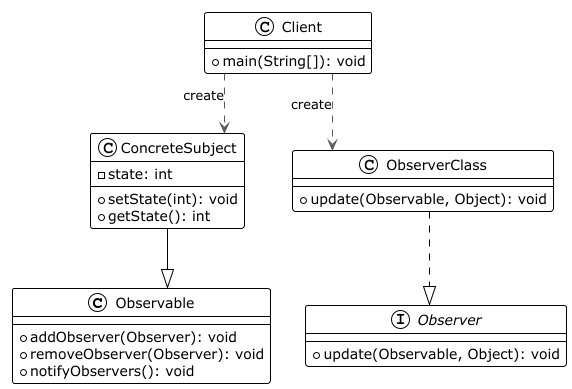
\includegraphics[width=0.5\textwidth]{ObserverUML}
                \caption{Struttura del pattern Observer}
            \end{figure}
        \subsubsection{Esempio}
\begin{lstlisting}{java}
public class ConcreteSubject extends Observable {
    private int state;
    public int getState() {
        return state;
    }
    public void setState(int state) {
        this.state = state;
        notifyObservers();
    }
}
public class ObserverClass implements Observer {
    @Override
    public void update(java.util.Observable o, Object arg) {
        System.out.println("ObserverClass.update()");
    }
}
public class Client {
    public static void main(String[] args) {
        ConcreteSubject subject = new ConcreteSubject();
        ObserverClass observer = new ObserverClass();
        subject.addObserver(observer);
        subject.setState(1);
    }
}
\end{lstlisting}
\subsection{Factory}
Il pattern Factory é un pattern creazionale che permette di creare oggetti senza specificare la classe esatta dell'oggetto che verrà creato,
viene utilizzato quando si vuole delegare la creazione di un oggetto a una classe Factory, questo consente di creare oggetti senza dover conoscere la logica di creazione.
\subsubsection{Struttura}
il pattern Factory é composto dai seguenti elementi:
\begin{itemize}
    \item \textbf{Product}: é l'interfaccia che definisce l'oggetto da creare.
    \item \textbf{ConcreteProduct}: é la classe concreta che implementa l'interfaccia Product.
    \item \textbf{Factory}: é l'interfaccia che definisce il metodo per creare l'oggetto.
    \item \textbf{ConcreteFactory}: é la classe concreta che implementa l'interfaccia Factory.
    \end{itemize}
\subsubsection{esempio}
\begin{lstlisting}[language=Java]
// Interfaccia Product
public interface Product {
    void operation();
}

// Classe concreta ConcreteProduct
public class ConcreteProduct implements Product {
    @Override
    public void operation() {
        System.out.println("ConcreteProduct.operation()");
    }
}

// Interfaccia Factory
public interface Factory {
    Product createProduct();
}

// Classe concreta ConcreteFactory
public class ConcreteFactory implements Factory {
    @Override
    public Product createProduct() {
        return new ConcreteProduct();
    }
}

// Classe Main per testare il pattern Factory
public class Main {
    public static void main(String[] args) {
        // Creazione della factory
        Factory factory = new ConcreteFactory();

        // Creazione del prodotto
        Product product = factory.createProduct();

        // Utilizzo del prodotto
        product.operation();
    }
}
\end{lstlisting}
\subsection{Singleton}
Il pattern Singleton é un pattern creazionale che permette di creare una sola istanza di una classe e fornire un punto di accesso globale a tale istanza.
\subsubsection{Struttura}
Il pattern Singleton é composto dai seguenti elementi:
\begin{itemize}
    \item \textbf{instance} : é l'attributo statico che contiene l'istanza della classe.
    \item \textbf{getInstance()} : é il metodo statico che restituisce l'istanza della classe.
    \item \textbf{costruttore privato} : é il costruttore privato che impedisce la creazione di nuove istanze della classe.
    \end{itemize}
\begin{figure}[H]
    \centering
    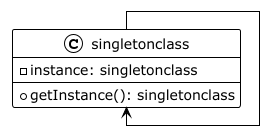
\includegraphics[width=0.5\textwidth]{singletonclass}
    \caption{Struttura del pattern Singleton}
\end{figure}
\subsubsection{esempio}
\begin{lstlisting}[language=Java]
public class Singleton {
    private static Singleton instance;

    private Singleton() {
    }

    public static Singleton getInstance() {
        if (instance == null) {
            instance = new Singleton();
        }
        return instance;
    }
}
\end{lstlisting}
\subsection{Decorator}
Il pattern Decorator consente di aggiungere nuovi comportamenti ad un oggetto legandolo ad un oggetto Decorator anche detto wrapper\footnote{Un wrapper è un oggetto che incapsula un altro oggetto per modificarne o estenderne il comportamento.},
in questo modo si può aggiungere funzionalità ad un oggetto senza doverlo modificare direttamente, inoltre il pattern Decorator permette di aggiungere o rimuovere funzionalità in maniera dinamica.
\newpage
\subsubection{Quando utilizzare il pattern Decorator}
Il pattern Decorator si utilizza quindi nei seguenti casi:
\begin{itemize}
    \item Quando si vuole aggiungere funzionalità ad un oggetto senza doverne modificare altri.
    \item Quando alcune funzionalità possono essere aggiunte o rimosse in maniera dinamica.
    \item Quando l' opzione di utilizzare l'ereditarietà per estendere le funzionalità di un oggetto non è possibile o non è conveniente.
    \end{itemize}
\subsubsection{Struttura del pattern Decorator}
Il pattern Decorator é quindi un pattern che si basa sul concetto di composizione, infatti l'oggetto concreto viene wrappato dalla
classe Decorator che a sua volta implementa l'interfaccia dell'oggetto concreto, in questo modo si possono aggiungere o rimuovere funzionalità,
inoltre il pattern Decorator permette di creare una gerarchia di Decorator che possono essere aggiunti in maniera dinamica.
per riassumere la struttura del pattern Decorator è composta dai seguenti elementi:
\begin{itemize}
    \item \textbf{Component}: è l'interfaccia che definisce l'oggetto che verrà wrappato.
    \item \textbf{ConcreteComponent}: è la classe concreta che implementa l'interfaccia Component.
    \item \textbf{BaseDecorator}: è la classe astratta che contiene al suo interno l'oggeto che fa uso dell'interfaccia concrete component.
    \item \textbf{ConcreteDecorator}: è la classe che estende BaseDecorator che aggiunge concretamente una funzionalitá.
\end{itemize}
\begin{figure}[h]
    \centering
    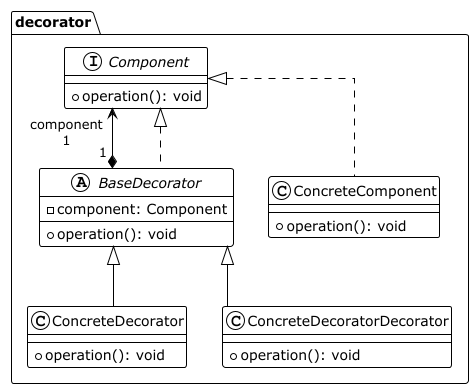
\includegraphics[width=0.5\textwidth]{decoratorUML}
    \caption{Struttura del pattern Decorator}
\end{figure}

\subsubsection{Esempio di utilizzo del pattern Decorator}
\begin{lstlisting}[language=Java]
// Definizione dell'interfaccia Component
public interface Component {
    void operation();
}

// Implementazione concreta del componente
public class ConcreteComponent implements Component {
    @Override
    public void operation() {
        System.out.println("ConcreteComponent operation");
    }
}

// Classe astratta BaseDecorator che implementa l'interfaccia Component
public abstract class BaseDecorator implements Component {
    protected Component component;

    // Costruttore che accetta un componente da decorare
    public BaseDecorator(Component component) {
        this.component = component;
    }

    // Metodo che chiama l'operazione del componente decorato
    @Override
    public void operation() {
        component.operation();
    }
}

// Implementazione concreta del decoratore
public class ConcreteDecorator extends BaseDecorator {
    public ConcreteDecorator(Component component) {
        super(component);
    }

    // Metodo che aggiunge un comportamento aggiuntivo
    @Override
    public void operation() {
        super.operation();
        System.out.println("ConcreteDecorator operation");
    }
}

// Implementazione concreta di un decoratore aggiuntivo
public class ConcreteDecoratorDecorator extends BaseDecorator {
    public ConcreteDecoratorDecorator(Component component) {
        super(component);
    }

    // Metodo che aggiunge un ulteriore comportamento aggiuntivo
    @Override
    public void operation() {
        super.operation();
        System.out.println("ConcreteDecoratorDecorator operation");
    }
}

// Classe Client per testare il pattern Decorator
public class Client {
    public static void main(String[] args) {
        // Creazione del componente concreto
        Component component = new ConcreteComponent();

        // Decorazione del componente con ConcreteDecorator
        Component decoratorA = new ConcreteDecorator(component);

        // Decorazione ulteriore del componente con ConcreteDecoratorDecorator
        Component decoratorB = new ConcreteDecoratorDecorator(decoratorA);

        // Esecuzione dell'operazione sul decoratore finale
        decoratorB.operation();
    }
}
\end{lstlisting}

\subsection{command pattern}
Il pattern command é un pattern comportamentale che permette di incapsulare una richiesta in un oggetto, in questo modo si può parametrizzare i client con diverse richieste, code o registri e supportare operazioni di undo,
inoltre il pattern command permette di separare il mittente dal ricevente, in questo modo si può inviare richieste a oggetti senza conoscere la loro implementazione.
\subsubsection{Struttura}
Il pattern command é composto dai seguenti elementi:
\begin{itemize}
    \item \textbf{Command}: é l'interfaccia che definisce il metodo per eseguire l'azione.
    \item \textbf{ConcreteCommand}: é la classe concreta che implementa l'interfaccia Command.
    \item \textbf{Invoker}: é la classe che invoca il comando.
    \item \textbf{Receiver}: é la classe che riceve il comando e lo esegue.
    \end{itemize}
\subsubsection{esempio}
\begin{lstlisting}[language=Java]
// Interfaccia Command
public interface Command {
    void execute();
}

// Implementazione concreta del comando
public class ConcreteCommand implements Command {
    private Receiver receiver;

    public ConcreteCommand(Receiver receiver) {
        this.receiver = receiver;
    }

    @Override
    public void execute() {
        receiver.action();
    }
}

// Classe Receiver
public class Receiver {
    public void action() {
        System.out.println("Receiver.action()");
    }
}

// Classe Invoker
public class Invoker {
    private Command command;

    public Invoker(Command command) {
        this.command = command;
    }

    public void execute() {
        command.execute();
    }
}

// Classe Main per testare il pattern Command
public class Main {
    public static void main(String[] args) {
        // Creazione del ricevente
        Receiver receiver = new Receiver();

        // Creazione del comando concreto
        Command command = new ConcreteCommand(receiver);

        // Creazione dell'invoker
        Invoker invoker = new Invoker(command);

        // Esecuzione del comando
        invoker.execute();
    }
}
\end{lstlisting}
\subsection{Builder}
Il pattern Builder é un pattern creazionale che permette di creare un oggetto complesso passo dopo passo, in questo modo si può creare un oggetto complesso senza dover creare un costruttore con un numero elevato di parametri.
\subsubsection{Struttura}
Il pattern Builder é composto dai seguenti elementi:
\begin{itemize}
    \item \textbf{Product}: é la classe che rappresenta l'oggetto complesso da costruire.
    \item \textbf{Builder}: é l'interfaccia che definisce i metodi per costruire l'oggetto.
    \item \textbf{ConcreteBuilder}: é la classe concreta che implementa l'interfaccia Builder.
    \item \textbf{Director}: é la classe che utilizza il Builder per costruire l'oggetto.
    \end{itemize}
\subsubsection{esempio}
\begin{lstlisting}[language=Java]
// Classe Product
public class Product {
    private String partA;
    private String partB;
    private String partC;

    public void setPartA(String partA) {
        this.partA = partA;
    }

    public void setPartB(String partB) {
        this.partB = partB;
    }

    public void setPartC(String partC) {
        this.partC = partC;
    }
}

// Interfaccia Builder
public interface Builder {
    void buildPartA();
    void buildPartB();
    void buildPartC();
    Product getProduct();
}

// Implementazione concreta del Builder
public class ConcreteBuilder implements Builder {
    private Product product;

    public ConcreteBuilder() {
        product = new Product();
    }

    @Override
    public void buildPartA() {
        product.setPartA("Part A");
    }

    @Override
    public void buildPartB() {
        product.setPartB("Part B");
    }

    @Override
    public void buildPartC() {
        product.setPartC("Part C");
    }

    @Override
    public Product getProduct() {
        return product;
    }
}

// Classe Director
public class Director {
    private Builder builder;

    public Director(Builder builder) {
        this.builder = builder;
    }

    public Product construct() {
        builder.buildPartA();
        builder.buildPartB();
        builder.buildPartC();
        return builder.getProduct();
    }
}

// Classe Main per testare il pattern Builder
public class Main {
    public static void main(String[] args) {
        // Creazione del Builder concreto
        Builder builder = new ConcreteBuilder();

        // Creazione del Director
        Director director = new Director(builder);

        // Costruzione del prodotto
        Product product = director.construct();
    }
}
\end{lstlisting}




\end{document}